%% Le lingue utilizzate, che verranno passate come opzioni al pacchetto babel. Come sempre, l'ultima indicata sarà quella primaria.
\def\thudbabelopt{italian,english} %% "english" is placed last to make it the primary language for the text.
%% Valori ammessi per target: bach (tesi triennale), mst (tesi magistrale), phd (tesi di dottorato).
%% Valori ammessi per aauheader: aics (Department of Artificial Intelligence and Cybersecurity)
\documentclass[target=mst,aauheader=aics,style=]{thud}

%% --- Informazioni sulla tesi ---
\course{Cybersecurity and Artificial Intelligence}
\title{Automated Threat Modeling Pipeline for Operational Technology Configurations using Declarative Logic Synthesis}
\author{Xhulia Palaj}
\supervisor{Prof.\ Marino Miculan}
\cosupervisor{Dr.\ Jasmin Wachter}
\tutor{Dott.\ Canzian}

%% --- Pacchetti consigliati ---
\usepackage[a-1b]{pdfx}
\usepackage[pdfa]{hyperref}
\usepackage{amsmath,amssymb}
\usepackage{booktabs}
\usepackage{listings}
\usepackage{xcolor}
\usepackage{tabularx}
\usepackage{tikz} 
\usetikzlibrary{shapes.geometric, arrows, positioning}

\lstdefinelanguage{yaml}{
  keywords={true,false,null,y,n},
  keywordstyle=\color{magenta},
  basicstyle=\ttfamily\footnotesize,
  sensitive=false,
  comment=[l]{\#},
  commentstyle=\color{codegreen},
  stringstyle=\color{codepurple},
  moredelim=[l][\color{magenta}]{\:},
  morestring=[b]',
  morestring=[b]"
}

% Define JSON syntax highlighting for listings
\lstdefinelanguage{json}{
    basicstyle=\ttfamily\footnotesize,
    showstringspaces=false,
    breaklines=true,
    frame=lines,
    backgroundcolor=\color{backcolour},
    literate=
     *{0}{{{\color{codepurple}0}}}{1}
      {1}{{{\color{codepurple}1}}}{1}
      {2}{{{\color{codepurple}2}}}{1}
      {3}{{{\color{codepurple}3}}}{1}
      {4}{{{\color{codepurple}4}}}{1}
      {5}{{{\color{codepurple}5}}}{1}
      {6}{{{\color{codepurple}6}}}{1}
      {7}{{{\color{codepurple}7}}}{1}
      {8}{{{\color{codepurple}8}}}{1}
      {9}{{{\color{codepurple}9}}}{1}
      {:}{{{\color{magenta}{:}}}}{1}
      {,}{{{\color{magenta}{,}}}}{1}
      {\{}{{{\color{magenta}{\{}}}}{1}
      {\}}{{{\color{magenta}{\}}}}}{1}
      {[}{{{\color{magenta}{[}}}}{1}
      {]}{{{\color{magenta}{]}}}}{1},
}

% Listing color styles
\definecolor{codegreen}{rgb}{0,0.6,0}
\definecolor{codegray}{rgb}{0.5,0.5,0.5}
\definecolor{codepurple}{rgb}{0.58,0,0.82}
\definecolor{backcolour}{rgb}{0.96,0.96,0.96}

\lstdefinestyle{mystyle}{
    backgroundcolor=\color{backcolour},   
    commentstyle=\color{codegreen},
    keywordstyle=\color{magenta},
    numberstyle=\tiny\color{codegray},
    stringstyle=\color{codepurple},
    basicstyle=\ttfamily\footnotesize,
    breakatwhitespace=false,         
    breaklines=true,                 
    captionpos=b,                    
    keepspaces=true,                 
    numbers=none,                    
    showspaces=false,                
    showstringspaces=false,
    showtabs=false,                  
    tabsize=2
}
\lstset{style=mystyle}

\begin{document}
\maketitle

%% Dedica (opzionale)
\begin{dedication}
    To be done in the end
\end{dedication}

%% Ringraziamenti (opzionali)
\acknowledgements
To be done in the end

%% Sommario (opzionale)
\abstract
To be done in the end

\tableofcontents

%% Corpo principale del documento
\mainmatter

% ==========================================
% CHAPTER 1: INTRODUCTION
% ==========================================
\chapter{Introduction}

\section{The Industrial Paradigm Shift \& Contextualizing OT Constraints}
Industrial Control Systems (ICS) and Operational Technology (OT) networks form the critical infrastructure backbone of contemporary manufacturing plants, power generation facilities, water treatment utilities, and heavy industrial operations \cite{SunderOT}. Historically, these architectures were physically isolated from external communications through dedicated air-gaps, relying on specialized hardware and vendor-proprietary, closed-loop protocols \cite{StanExtended}. However, the rapid acceleration of Industry 4.0 paradigms, Industrial Internet of Things (IIoT) platforms, and centralized manufacturing telemetry has forced a widespread structural convergence between corporate Information Technology (IT) enterprise networks and operational production environments.

While this interconnectivity facilitates real-time supply-chain analytics and automated resource management, directly porting enterprise IT security frameworks into operational technology ecosystems introduces profound systemic friction due to fundamentally opposing operational priorities. In enterprise IT ecosystems, cybersecurity architectures are governed by the classical CIA Triad (Confidentiality, Integrity, and Availability), wherein data-at-rest encryption, data-in-transit privacy, and access control policies take precedence over operational continuity. 

Within Operational Technology, this hierarchy undergoes a complete structural inversion, transitioning into a paradigm governed by continuous availability, deterministic loop execution, and human/physical safety \cite{SunderOT}. An unauthorized data exposure within an enterprise IT environment incurs regulatory penalties or financial liabilities, but an unplanned shutdown, delayed control loop, or buffer fault in an industrial automation plant can precipitate catastrophic kinetic failures, physical equipment destruction, environmental disasters, and fatal occupational hazards. As a result, standard enterprise strategies---such as routine intrusive vulnerability scanning, automated operating system patching, and reactive fail-closed network terminations---cannot be safely executed on active production lines.

\section{The Economic and Physical Risks of Active Vulnerability Testing}
Because industrial automation assets---such as Human-Machine Interfaces (HMIs), Programmable Logic Controllers (PLCs), Remote Terminal Units (RTUs), and Supervisory Control and Data Acquisition (SCADA) servers---frequently run legacy embedded software stacks, they exhibit acute structural fragility \cite{SunderOT}. Standard IT risk management practices rely heavily on active network scanners (e.g., Nessus, OpenVAS, aggressive Nmap service sweeps) to probe ports, transmit malformed request packets, and extract service banners to map known software Common Vulnerabilities and Exposures (CVEs) \cite{Ou05}.

In an operational technology environment, the high volume of socket connections, unexpected payload formats, and high-frequency packet rates generated by active scanners can instantly overwhelm the single-threaded compute engines and finite memory buffers of legacy embedded field devices. This buffer exhaustion can force PLCs into fatal hardware fault modes, disrupt cycle times, or induce control-loop blindness in SCADA monitoring systems. 

Given that unplanned downtime in capital-intensive heavy industries (such as automated steel manufacturing, chemical refining, and automotive production) incurs severe financial penalties and risks hardware damage, live active penetration testing and intrusive scanning cannot be performed on running environments \cite{TayouriSurvey}. Instead, comprehensive threat assessments, predictive vulnerability modeling, and mitigation strategies must be conducted entirely out-of-band using formal, non-disruptive mathematical modeling prior to physical plant commissioning or maintenance cycles.

\section{Limitations of Manual Risk Analysis in Large-Scale Industrial Automation}
Modern industrial manufacturing environments are vast, highly heterogeneous, and structurally complex. These infrastructures are strictly segmented across network layers defined by the ANSI/ISA-95 Purdue Reference Model, incorporating:
\begin{itemize}
    \item Dozens of virtualized supervisory nodes, engineering workstations (EWS), domain controllers, and process historians operating across Level 3 and Demilitarized Zones (DMZ) \cite{SunderOT}.
    \item Distributed client-server Human-Machine Interfaces (HMIs) and manufacturing execution management servers interacting across isolated physical process cells.
    \item Enterprise-wide Active Directory (AD) forests and identity management services managing plant-wide administrative credentials.
    \item Hundreds of embedded Level 1 PLCs communicating directly with field-level Level 0 actuators, variable frequency drives, and sensors via unauthenticated fieldbus networks \cite{StanExtended}.
\end{itemize}

Evaluating the threat surface of a facility of this scale through manual security audits is inefficient, mathematically incomplete, and error-prone \cite{KonstaSurvey}. Manual auditing teams routinely evaluate assets in isolation, failing to evaluate non-obvious, multi-stage attack paths created by intersecting firewall exceptions, cross-zone routing rules, and systemic credential reuse. 

To overcome these manual limitations, the automated synthesis of Logical Attack Graphs (LAGs) is essential \cite{Ou05, TayouriMIRAGE}. By synthesizing network topologies, access control lists (ACLs), host software profiles, and industrial protocol properties into formal declarative logic, automated verification engines can mathematically prove how an adversary can enter the perimeter, pivot through intermediate supervisory layers, exploit legacy protocol flaws, and achieve lateral movement to compromise physical industrial processes.

\section{Objectives and Core Scope of the Thesis Research}
The primary objective of this thesis research is to design, implement, and evaluate an automated, non-intrusive threat modeling pipeline capable of ingesting raw, human-managed industrial configuration inventories, translating them into formal declarative logic representations, and generating multi-stage logical attack paths threatening critical plant controllers \cite{Ou05}.

To bridge the gap between semi-structured configuration metadata and formal mathematical reasoning engines, this study establishes an end-to-end framework organized around four research pillars:
\begin{enumerate}
    \item \textbf{Configuration Ingestion \& Normalization:} Developing an ingestion layer to extract asset identities, operating system parameters, listening services, and firewall access control matrices directly from production JSON configuration files \cite{TayouriMIRAGE}.
    \item \textbf{Neuro-Symbolic Logic Synthesis:} Evaluating advanced knowledge extraction methods, combining Large Language Models (LLMs) with Answer Set Programming (ASP) and Horn-clause Datalog solvers, to automate the translation of raw network states into formally verified logic facts without the brittleness of deterministic parsers \cite{alviano2025llmasp}.
    \item \textbf{Domain-Specific OT Logic Modeling:} Extending standard vulnerability analysis engines (specifically MulVAL) with custom interaction rules capable of capturing Purdue Reference Model constraints, unauthenticated legacy automation protocols (Modbus/TCP, PROFINET), and lateral credential reuse \cite{StanExtended, SunderOT}.
    \item \textbf{Adversary Mapping \& Mitigation Guidance:} Correlating derived logical attack paths directly with real-world adversary tactics and techniques established in the MITRE ATT\&CK for ICS knowledge base to generate actionable hardening recommendations and counterfactually verify risk reduction \cite{mitre_ics}.
\end{enumerate}

Through empirical testing on an industrial production topology, this thesis demonstrates a scalable, production-grade model to evaluate complex Operational Technology network configurations securely, efficiently, and with zero operational disruption.

% ==========================================
% CHAPTER 2: BACKGROUND
% ==========================================
\chapter{Background}

\section{Attack Trees, Logical Attack Graphs, and Symbolic Representations}

\subsection{The Limitations of Traditional Graph-Theoretic State-Space Models}
The early formalization of automated security analysis in networked environments relied on state-space transition systems \cite{KonstaSurvey}. In these models, security analysis was treated as a verification problem where the entire network infrastructure was modeled as a global finite state machine. Each node in the graph represented an explicit, global snapshot of the network, capturing the exact operating system state, patch levels, open ports, and active privilege levels across every host simultaneously. Edges between these state nodes represented discrete atomic state transitions, such as an adversary executing an exploit to transition the network from one global state to another.

While conceptually straightforward, state-space transition systems suffer from a severe computational limitation known as \textit{state-space explosion} \cite{Ou05}. Because these frameworks attempt to track all global state permutations, the size of the state graph scales exponentially with the number of networked assets and associated vulnerabilities. For a network containing $H$ distinct hosts, where each host can occupy one of $S$ distinct security configurations, the theoretical state space expands to:
\begin{equation}
|\mathcal{S}| = O(S^H)
\end{equation}

When applied to enterprise-scale industrial automation infrastructures---which often comprise hundreds of virtual machines, distributed HMIs, engineering workstations, and embedded PLCs---computing the full state transition graph quickly exceeds processing and memory limits \cite{KonstaSurvey}. This computational bottleneck makes real-time, dynamic risk assessment mathematically unfeasible under a state-space architecture.

\subsection{Shift to the Monotonic Logic Paradigm and Horn-Clause Datalog}
To bypass the exponential overhead of state-space exploration, modern predictive security modeling transitioned to a formal logic programming paradigm \cite{Ou05}. Pioneered by frameworks like MulVAL (Multi-host, Multi-stage Vulnerability Analysis Language), this methodology reformulates threat analysis from state-space searching into declarative theorem proving. Rather than tracking global system states, a logic-based model represents the network through declarative clauses expressed in a subset of first-order logic known as Horn-clause Datalog.

A Horn clause is a disjunction of literals containing at most one positive literal, typically written in rule format as:
\begin{equation}
H \leftarrow B_1 \land B_2 \land \dots \land B_m
\end{equation}
where the head $H$ is derived as a logical consequence if all body subgoals $B_1, \dots, B_m$ are satisfied \cite{Ou05}.

This paradigm shift relies fundamentally on the principle of \textit{monotonicity}. In a monotonic logic framework, it is assumed that an adversary's acquired privileges and network reachability accumulate over time and are never revoked during the evaluated attack sequence \cite{Ou05}. If an attacker acquires administrative control over a jump server, that privilege remains a true logical fact throughout the duration of the multi-stage evaluation.

By treating attack graph generation as a monotonic derivation problem over Horn clauses, the reasoning engine eliminates the need to maintain a combinatorial graph of explicit system states. Consequently, the computational complexity of attack path synthesis is drastically reduced from exponential time to polynomial time $O(N^2)$, where $N$ represents the total number of independent configuration facts, reachability predicates, and vulnerability assertions in the knowledge base \cite{Ou05}.

\subsection{Taxonomies of Automated Attack Generation Methodologies}
In their comprehensive methodological surveys, Konsta et al. categorize automated attack modeling frameworks into three primary generation paradigms \cite{KonstaSurvey}:
\begin{itemize}
    \item \textbf{Pure Graph-Theoretic Architectures:} These systems construct explicit directed graphs to map paths, relying on graph traversal algorithms (e.g., Dijkstra, Breadth-First Search) to evaluate reachability. While effective for small networks, they remain limited by state-space explosion when applied to complex topologies.
    \item \textbf{Model-Checking Frameworks:} Leveraging formal verification engines such as NuSMV or SPIN, these approaches model network components as strict state machines and use temporal logic formulas (e.g., LTL or CTL) to verify safety properties. While mathematically rigorous, they demand substantial memory in large infrastructures.
    \item \textbf{Rule-Based Declarative Logic Engines:} Frameworks such as MulVAL leverage Horn-clause logic programming and backward-chaining engines to evaluate security risks \cite{Ou05}. This architecture provides scalability and expressiveness by abstracting network configurations into static relational facts and generic interaction rules, though natively maintaining a static, monotonic view of the environment.
\end{itemize}

\subsection{Algorithmic Path Discovery \& Scalability Considerations}
As network infrastructures expand to encompass hundreds of interconnected enterprise and operational assets, the total volume of ground configuration facts grows proportionally \cite{AbdellatifAAPDEM}. While monotonic Horn-clause Datalog solvers operate in polynomial time $O(N^2)$, evaluating thousands of rules and predicates across complex corporate-to-OT boundaries can yield extensive derivation trees.

To address computational overhead in massive topologies, recent literature has explored specialized path optimization heuristics, including cost-aware $A^*$ search algorithms (such as the AAPDEM model \cite{AbdellatifAAPDEM}), Deep Reinforcement Learning (DRL) pathfinding agents, and Graph Neural Networks (GNNs) evaluating temporal automata properties \cite{StammetGNN}. While these learning-based models provide value for rapid path pruning in hyper-scale cloud environments, they introduce trade-offs in verification explainability and completeness.

In safety-critical industrial automation plants, exhaustive completeness and deterministic formal soundness are mandatory requirements \cite{SunderOT}. Because industrial plant topologies (comprising dozens of servers, engineering workstations, and Level 1 PLCs) remain well within the polynomial scaling envelope of Datalog engines, this research adopts exhaustive, goal-directed backward-chaining powered by XSB Prolog tabling (memoization) \cite{swift2012xsb}. Tabling eliminates redundant re-evaluations and guarantees that all possible adversarial propagation routes are identified deterministically.

\subsection{Software Bill of Materials (SBOM) and Modern Asset Manifests}
In modern industrial cybersecurity engineering, tracking installed software components across heterogeneous devices increasingly relies on standardized Software Bill of Materials (SBOM) manifests \cite{cyclonedx, spdx}. Standards such as CycloneDX (OWASP) and SPDX (ISO/IEC 5962) structure package identifiers, version hierarchies, and cryptographic component hashes into machine-readable JSON or XML documents. 

In Operational Technology, asset configuration dumps (such as the \texttt{configuration.json} schema targeted in this work) serve as macroscopic plant-level manifests. Integrating SBOM-aligned parsing principles ensures that embedded daemons, firmware versions, and communication interfaces are extracted with high fidelity, establishing an explicit bridge to vulnerability intelligence feeds \cite{cyclonedx}.

\subsection{Adversary Modeling via the MITRE ATT\&CK for ICS Matrix}
To evaluate industrial cyber-threats beyond abstract reachability graphs, modern security engineering benchmarks attack trajectories against standardized adversary behavioral frameworks \cite{mitre_ics}. Developed specifically to capture operational technology threat vectors, the \textbf{MITRE ATT\&CK for ICS} knowledge base categorizes real-world adversary actions across fourteen distinct tactics, spanning \textit{Initial Access}, \textit{Execution}, \textit{Persistence}, \textit{Privilege Escalation}, \textit{Evasion}, \textit{Lateral Movement}, \textit{Inhibit Response Function}, and \textit{Impair Process Control}.

Unlike enterprise IT attack matrices that emphasize data exfiltration and identity harvesting, ATT\&CK for ICS formalizes domain-specific techniques such as unauthorized command message injection (T0855), controller firmware modification (T0890), and parameter manipulation of physical equipment (T0836) \cite{mitre_ics}. Correlating formal logic interaction rules directly with ATT\&CK for ICS techniques provides a standardized methodology to translate mathematical attack graph proofs into actionable defense-in-depth mitigations.

\section{MulVAL Engine Architecture \& Execution Semantics}
The core execution architecture of MulVAL achieves high scalability by separating the threat model into two distinct, decoupled components: Static Configuration Facts and Generic Interaction Rules \cite{Ou05}.

\subsection{Static Configuration Facts}
These represent the immutable, factual configuration of the target network environment \cite{Ou05}. They are expressed as ground Datalog clauses that register network topology, firewall access control lists (ACLs), software installations, and software vulnerabilities:
\begin{itemize}
    \item \texttt{located(Host, Subnet, Type)}: Maps the network topology placement and subnet boundary of an asset.
    \item \texttt{networkService(Host, Program, Protocol, Port, Privilege)}: Defines a listening service binding, port number, and its local execution permissions.
    \item \texttt{vulHost(Host, CVE, Program, ExploitType, Consequence)}: Binds vulnerability intelligence and exploitation consequences to specific hosts.
    \item \texttt{aclNW(Source, Destination, Protocol, Port)}: Represents network filtering, routing reachability, and firewall policies.
\end{itemize}

\subsection{Generic Interaction Rules}
These rules act as the underlying mathematical "adversarial physics" that dictate how an attacker can propagate through an environment \cite{Ou05}. These are written as abstracted Horn clauses that define the conditions under which a new logical deduction can be derived from existing facts. For example, a standard remote exploit interaction rule is defined as:
\begin{equation}
\begin{aligned}
\text{execCode}(\text{Target}, \text{Priv}) \leftarrow \; & \text{networkService}(\text{Target}, \text{Prog}, \text{Prot}, \text{Port}, \text{Priv}), \\
& \text{vulHost}(\text{Target}, \text{CVE}, \text{Prog}, \text{remoteExploit}, \text{privEscalation}), \\
& \text{netAccess}(\text{Principal}, \text{AttackerHost}, \text{Target}, \text{Prot}, \text{Port}).
\end{aligned}
\end{equation}

\subsection{The Derivation Engine and Table Optimization}
MulVAL utilizes an underlying XSB Prolog execution engine to perform goal-directed, backward-chaining derivation \cite{swift2012xsb}. Given a user-defined target condition---such as \texttt{attackGoal(unauthorizedControl(plc\_l1\_1))}---the engine resolves backward, evaluating which combinations of interaction rules and configuration facts can satisfy the terminal objective.

To optimize this process and prevent non-terminating loops caused by cyclic network dependencies (such as two hosts running identical software and sharing reciprocal network access), the engine leverages XSB Tabling Optimization Directives (e.g., \texttt{:- table execCode/2.}) \cite{swift2012xsb}. Tabling enforces memoization: once a specific security subgoal is evaluated, its truth value is cached in an internal lookup table. If the engine encounters the same subgoal later in another branch of the attack tree, it retrieves the cached result instantly rather than re-evaluating the entire logic sequence. This ensures that the engine dynamically constructs a comprehensive Logical Attack Graph (LAG) while maintaining low polynomial computation times \cite{Ou05}.

\section{The Neuro-Symbolic Ingestion Paradigm (LLMASP Integration)}
While logic-based vulnerability analysis engines provide a scalable framework for evaluating multi-stage attack paths, an automation gap remains in the initial ingestion pipeline \cite{KonstaSurvey}. The MulVAL reasoning engine relies on declarative Datalog clauses to model network state \cite{Ou05}. However, real-world operational environments do not maintain their configurations or asset inventories as mathematical predicates; instead, network states and software inventories exist as semi-structured JSON profiles, spreadsheets, or configuration logs \cite{SunderOT}.

To automate this knowledge extraction without relying on brittle, hardcoded regular expression scripts, this research integrates a neuro-symbolic approach based on the LLMASP framework introduced by Alviano et al. (IJCAI 2025) \cite{alviano2025llmasp}.

LLMASP establishes a dual-process neuro-symbolic division of labor based on cognitive theory:
\begin{itemize}
    \item \textbf{System-1 (LLM / Syntactic Extraction):} Large Language Models excel at natural language comprehension, pattern recognition, and syntactic entity extraction. In this architecture, the LLM is restricted strictly to syntactic parsing, converting semi-structured JSON objects into explicit Datalog atom strings based on structured prompt specifications.
    \item \textbf{System-2 (Answer Set Programming / Formal Reasoning):} ASP solvers (e.g., Clingo) operate over declarative Horn clauses and disjunctive logic programs under stable model semantics \cite{clingo}. The ASP engine processes background knowledge rules to infer implicit network relationships (such as credential-sharing links and unauthenticated protocol bindings), verify type constraints, and eliminate logical inconsistencies before facts are submitted to MulVAL.
\end{itemize}

By restricting the LLM to syntactic translation and offloading logical deduction to an ASP/Datalog engine, the framework mitigates generative hallucinations, prevents predicate arity mismatches, and guarantees compile-time logical soundness \cite{alviano2025llmasp}.

\section{MIRAGE: Micro-Level Firmware Vulnerability Modeling}
\label{sec:mirage_detailed_background}

\subsection{Multi-Binary Firmware Vulnerability Context}
In recent embedded device security research, the MIRAGE (Multi-Binary Image Risk Assessment with Attack Graph Employment) framework introduced by Tayouri et al. represents a foundational milestone in extending Logical Attack Graphs (LAGs) beyond conventional IT networks \cite{TayouriMIRAGE}. 

Traditional vulnerability assessment tools analyze IoT and embedded OT edge devices as monolithic entities \cite{TayouriMIRAGE}. However, modern embedded devices run multi-binary embedded Linux distributions (e.g., OpenWrt, BusyBox environments) where operational tasks---such as HTTP web servers, UPnP daemons, DNS forwarders, and proprietary industrial protocol parsers---are partitioned across disparate executable binaries. These distinct binaries execute concurrently under varying privilege boundaries and communicate internally via Inter-Process Communication (IPC) channels, including UNIX domain sockets, FIFO named pipes, shared memory segments, and environment variables.

Tayouri et al. demonstrated that evaluating vulnerabilities within isolated binaries produces severe blind spots \cite{TayouriMIRAGE}. An adversary who successfully exploits an initial memory corruption bug in an exposed, network-facing binary (e.g., a lightweight web server) rarely achieves direct root execution immediately. Instead, the attacker initiates an \textit{intranode lateral pivot}: by manipulating local IPC data streams or exploiting shared dynamic libraries (e.g., vulnerable \texttt{libuClibc} routines), the adversary propagates execution across internal binary boundaries, progressively escalating privileges until full device takeover is achieved.

\subsection{The Four-Stage MIRAGE Architecture}
To model intra-device vulnerability chaining, MIRAGE structures risk assessment into a sequential four-stage static analysis pipeline \cite{TayouriMIRAGE}:
\begin{enumerate}
    \item \textbf{Binary Modeler (Firmware Decomposition):} Unpacks compressed firmware filesystem images (SquashFS, CramFS, JFFS2) using Binwalk. It performs static analysis to chart border binaries (daemons bound to external TCP/UDP sockets) and maps internal IPC data dependencies across local binaries.
    \item \textbf{Vulnerability Mapper (NVD Heuristics \& QEMU Emulation):} Identifies software Common Vulnerabilities and Exposures (CVEs) affecting individual binaries. It queries the NIST National Vulnerability Database (NVD) using static indicator heuristics, version string scraping, and QEMU-emulated command-line execution (e.g., parsing binary banner flags) to emit \texttt{vulExists/5} predicates.
    \item \textbf{Attack Graph Generator (Intranode Logic Engine):} Ingests extracted IPC dependencies and \texttt{vulExists} assertions into an extended MulVAL engine. MIRAGE defines specialized interaction rules that formalize how memory corruption in one binary transfers tainted control flow to adjacent binaries over local IPC channels.
    \item \textbf{Attack Graph Analyzer (EPSS Risk Scoring):} Computes risk scores across derived attack paths by combining binary interaction frequency (impact) with the Exploit Prediction Scoring System (EPSS) probability metrics (likelihood).
\end{enumerate}

\subsection{Theoretical and Methodological Disconnect: Why MIRAGE Differs from Our Goals}
While MIRAGE successfully applied MulVAL attack graphs to embedded firmware, its architecture cannot be ported directly to solve the threat modeling challenge targeted in this thesis. A fundamental methodological, structural, and semantic gap exists between MIRAGE's micro-level firmware objectives and our macroscopic industrial plant requirements. 

Table~\ref{tab:mirage_comparative_detailed} formalizes the multidimensional comparison between the MIRAGE baseline and our proposed neuro-symbolic framework.

\begin{table}[htbp]
\centering
\small
\caption{Comprehensive Methodological Comparison: MIRAGE Micro-Firmware Baseline vs. Our Industrial Macro Threat Pipeline}
\label{tab:mirage_comparative_detailed}
\begin{tabularx}{\textwidth}{p{0.22\textwidth}Xp{0.38\textwidth}}
\toprule
\textbf{Dimensional Axis} & \textbf{MIRAGE Firmware Baseline \cite{TayouriMIRAGE}} & \textbf{Our Macro-Industrial Framework} \\
\midrule
\textbf{Target Scope \& Abstraction} & 
\textbf{Micro-Level (Single Device):} Evaluates internal execution boundaries across separate binaries within a single compressed firmware image. & 
\textbf{Macro-Level (Plant Footprint):} Evaluates multi-tier Purdue Model architectures spanning 21+ virtualized servers, domain controllers, PLCs, and physical drives \cite{SunderOT}. \\
\addlinespace
\textbf{Communication Boundary} & 
\textbf{Intra-Node IPC Channels:} UNIX domain sockets, named pipes, shared memory, and environment variables. & 
\textbf{Inter-Zone Network ACLs:} Multi-tier firewall packet filtering matrices (\texttt{aclNW/4}) and layer-2 fieldbuses (\texttt{l2Connection/5}). \\
\addlinespace
\textbf{Input Artifact \& Ingestion} & 
\textbf{Filesystem Images:} Decompressed via Binwalk; relies on static string heuristics and rigid regex matching. & 
\textbf{Semi-Structured Configs:} Ingests production JSON asset sheets via LLMASP (System-1 neural extraction + System-2 ASP completion) \cite{alviano2025llmasp}. \\
\addlinespace
\textbf{Vulnerability Spectrum} & 
\textbf{Pure Software CVEs:} Evaluates memory corruption bugs in software binaries cataloged in NVD via CVSS/EPSS lookups. & 
\textbf{Hybrid Dual-Class Model:} Combines software CVEs (Class~I) with exploitless protocol flaws (Modbus/PROFINET) and credential reuse (Class~II) \cite{StanExtended}. \\
\addlinespace
\textbf{Deductive Rule Logic} & 
\textbf{Binary Taint Chaining:} Models privilege transfer across local processes via shared dynamic libraries (\texttt{libuClibc}). & 
\textbf{Purdue Zone Traversal:} Models multi-hop lateral movement, Active Directory domain takeover, and fieldbus master-slave hijacking. \\
\addlinespace
\textbf{Terminal Attack Goals} & 
\textbf{Local OS Privilege:} Hijacking root execution context inside the target device operating system. & 
\textbf{Kinetic Disruption:} \texttt{domainCompromise}, \texttt{unauthorizedControl}, and \texttt{physicalDriveControl}. \\
\addlinespace
\textbf{Actionable Output} & 
\textbf{Risk Metrics:} Generates numerical EPSS/CVSS scores and binary risk priority counts. & 
\textbf{Counterfactual Hardening:} Generates MITRE ATT\&CK for ICS remediations and verifies attack tree collapse upon patch simulation \cite{mitre_ics}. \\
\bottomrule
\end{tabularx}
\end{table}

\subsection{Key Disconnect Points Explained}
Analyzing the structural divergence between these two frameworks reveals five critical reasons why our research required an entirely distinct neuro-symbolic architecture:

\begin{enumerate}
    \item \textbf{Spatial Abstraction (Intra-Device vs. Inter-Zone):} MIRAGE operates within the execution space of a single microcontroller or system-on-chip (SoC) \cite{TayouriMIRAGE}. Its "network" is the Linux kernel's IPC table. In contrast, heavy industrial manufacturing facilities operate across distinct physical and virtual subnets strictly segmented by industrial firewalls under the Purdue Model \cite{SunderOT}. The security problem is not how \texttt{httpd} communicates with \texttt{dnsmasq}, but how an adversary on an external DMZ jump server traverses supervisory zones to inject unauthorized commands into a Level 1 PLC.

    \item \textbf{Ingestion Paradigm (Binary Unpacking vs. Neuro-Symbolic Synthesis):} MIRAGE relies on Binwalk to extract static binaries from firmware filesystems \cite{TayouriMIRAGE}. In production industrial plants, security teams do not possess the source firmware binaries for dozens of proprietary, vendor-locked PLCs (e.g., Danieli Automation DACI, Siemens S7-1500). Instead, security analysts manage high-level configuration management databases (CMDBs), firewall access tables, and network asset inventories stored as semi-structured JSON objects \cite{SunderOT}. Our framework bridges this representation by adopting the LLMASP neuro-symbolic paradigm \cite{alviano2025llmasp}, decoupling inductive neural parsing from Answer Set Programming completion.

    \item \textbf{Vulnerability Taxonomy (Exploits vs. Insecure-by-Design Protocols):} MIRAGE assumes that all adversarial propagation is driven by standard software implementation flaws (CVEs) cataloged in the NVD \cite{TayouriMIRAGE}. In operational technology, this assumption fails completely: Level 1 controllers and Level 0 fieldbus drives are routinely compromised without exploiting any software memory vulnerabilities \cite{StanExtended}. Field protocols (Modbus/TCP, PROFINET) lack authentication by design. While MIRAGE maps strictly to \texttt{vulExists/5}, our framework establishes a **Dual-Class Vulnerability Engine** that treats unauthenticated protocols and systemic administrative password reuse as first-class logical derivation primitives \cite{StanExtended, SunderOT}.

    \item \textbf{Dynamic Lookups vs. Deterministic Logical Isolation:} MIRAGE performs live, dynamic NVD queries and QEMU-emulated banner checks during pipeline execution \cite{TayouriMIRAGE}. In our framework, vulnerability data enters the deductive reasoning phase as pre-classified 5-tuples. The CVE identifier string is logically inert and serves exclusively as a descriptive annotation label within the generated attack graph, ensuring that the formal soundness of the derivation tree is decoupled from external API availability \cite{Ou05}.

    \item \textbf{Operational Impact (Device Root vs. Kinetic Plant Disruption):} For MIRAGE, the terminal objective is achieving administrative execution on the device OS \cite{TayouriMIRAGE}. In heavy industrial automation, an operating system compromise is merely an intermediate stepping stone \cite{SunderOT}. The ultimate threat is physical equipment damage, process downtime, and operator hazard resulting from unauthorized physical drive actuation or sensor telemetry tampering \cite{StanExtended}.
\end{enumerate}

Thus, while our research adopts the elegant **four-stage organizational shape** pioneered by MIRAGE (asset modeling $\to$ vulnerability mapping $\to$ interaction derivation $\to$ path analysis) \cite{TayouriMIRAGE}, the underlying computational machinery, spatial abstraction, and logical rules are realigned from micro-level firmware filesystems to macroscopic, multi-tier industrial plant networks \cite{Ou05, alviano2025llmasp, SunderOT}.

\section{OT Networks and the Purdue Reference Model}
To isolate fragile automation equipment from volatile business enterprise networks, industrial architectures are structured according to the Purdue Reference Model for ICS Security (ANSI/ISA-95) \cite{SunderOT}. This hierarchical architecture organizes industrial plant networks into distinct operational zones:
\begin{itemize}
    \item \textbf{Level 4 / Enterprise Network:} Hosts enterprise resource planning (ERP), corporate database systems, and business management services.
    \item \textbf{Level 3.5 / Industrial DMZ (IDMZ):} Provides a security barrier containing jump servers, reverse proxies, and patch management servers to terminate direct network sessions between enterprise and automation environments.
    \item \textbf{Level 3 / Operations Management:} Houses plant-wide supervisory control servers, data historians, engineering workstations (EWS), and domain controllers managing operational authorization.
    \item \textbf{Level 2 / Control Systems:} Encompasses supervisory control networks, local Human-Machine Interfaces (HMIs), and localized SCADA operator terminals.
    \item \textbf{Level 1 / Basic Control:} Contains Programmable Logic Controllers (PLCs), Remote Terminal Units (RTUs), and safety instrumented systems executing real-time control algorithms.
    \item \textbf{Level 0 / Physical Process:} Comprises physical actuators, sensors, motors, variable frequency drives, and physical field instrumentation.
\end{itemize}

Traditional logic engines treat network topologies as flat, interconnected graphs or simple point-to-point connections \cite{Ou05}. To build a mathematically precise model of an industrial facility, the Datalog engine must enforce these Purdue boundaries using explicit structural facts \cite{SunderOT}:
\begin{lstlisting}[language=Prolog]
located(jump_server, ot_dmz, ipSubnet).
located(vdc01, enterprise_mgt, ipSubnet).
located(ews_workstation, level_2_supervisory, ipSubnet).
located(plc_l1_1, level_1_control, ipSubnet).
located(drive_area_1_1, level_0_fieldbus, l2Bus).
\end{lstlisting}

By explicitly declaring these operational boundaries, the reasoning engine can enforce perimeter-crossing constraints, modeling how an adversary positioned at an external perimeter must pivot through intermediate supervisory zones before reaching critical Level 1 control assets \cite{SunderOT}.

\section{Domain-Specific Logic Extensions for Cyber-Physical Systems}
While foundational logic engines like MulVAL revolutionized automated threat modeling, their standard rule sets are inherently constrained to traditional IT abstractions \cite{Ou05, StanExtended}. In a standard IT security model, system interactions are generalized around standard operating system permissions (e.g., \texttt{user}, \texttt{admin}, \texttt{root}), network connections established over standard TCP/IP sockets, and software vulnerabilities cataloged exclusively via the CVE index.

However, this abstraction fails when applied to the operational realities of Cyber-Physical Systems (CPS) \cite{StanExtended, SunderOT}. Industrial environments incorporate thousands of embedded field devices that lack standard operating systems or user account management. In these networks, compromise does not merely manifest as user-to-root privilege escalation; instead, it frequently involves the unauthorized injection of unauthenticated control commands directly into a physical process loop. To capture realistic multi-stage adversarial pathways within industrial infrastructures, formal logic threat models must be extended with domain-specific interaction rules that natively capture network hierarchies, industrial protocol behaviors, and cyber-physical dependencies \cite{StanExtended, SunderOT}.

\section{MulVAL's Limitations in Industrial Environments}
Standard vulnerability scanners and IT-centric logic engines exhibit blind spots when analyzing industrial network configurations \cite{SunderOT}:
\begin{enumerate}
    \item \textbf{Individual Asset Assessment:} They evaluate assets in isolation, assuming that the absence of a known software CVE equates to a secure operational state \cite{Ou05}.
    \item \textbf{Flat Topology Assumptions:} Traditional logic engines treat network filtering policies as simple end-to-end reachability checks, failing to capture the cascading consequences that zone-to-zone firewall policies impose across multi-tier Purdue layers \cite{SunderOT}.
    \item \textbf{Protocol Blindness:} Traditional IT logic structures lack predicates to express the unauthenticated and unencrypted landscape of legacy industrial communications pervasive across lower architectural layers \cite{StanExtended}.
\end{enumerate}

\section{Modeling Legacy Industrial Protocols and Exploitless Vulnerabilities}
A critical security risk in OT environments stems from the pervasive reliance on legacy automation protocols---such as Modbus/TCP, PROFINET, and EtherNet/IP---which were designed without cryptographic authentication, integrity checks, or encryption \cite{StanExtended, SunderOT}. Consequently, any network node that achieves logical or physical proximity to an industrial bus can execute entirely exploitless compromises, such as spoofing control messages, rewriting PLC register parameters, or issuing force-shutdown commands to field devices.

To capture these protocol characteristics within a formal logic framework, the threat model introduces custom interaction rules representing vulnerabilities in the communication protocol itself, rather than software implementation errors (CVEs) \cite{StanExtended}:
\begin{lstlisting}[language=Prolog]
vulLinkProtocol(sub_proc_area_1, vul_modbus_no_auth, modbus, adjacent, impersonateDst).
\end{lstlisting}

When an adversary achieves network reachability to an unauthenticated controller port, the logic engine evaluates this as an immediate command injection pathway:
\begin{lstlisting}[language=Prolog]
interaction_rule(
  (unauthorizedControl(TargetPLC) :-
    execCode(SupervisorHost, admin),
    aclNW(SupervisorHost, TargetPLC, tcp, 502),
    networkService(TargetPLC, _Service, tcp, 502, _Perm)),
  rule_desc('Unauthorized command injection into PLC over unauthenticated Modbus/TCP', 0.9)
).
\end{lstlisting}

This extended rule allows the engine to mathematically prove how a compromised engineering workstation or administrative jump server can bypass traditional security barriers and manipulate physical field equipment directly over unauthenticated operational buses \cite{StanExtended, SunderOT}.

\section{Access Control Matrices and Zone-to-Zone Cross-Talk Logic}
Because network segmentation via industrial firewalls represents the primary line of defense in an OT infrastructure, the logic model enforces a strict network filtering matrix \cite{SunderOT}. In an industrial plant, network access is constrained: assets in a Level 2 supervisory network are restricted from interacting directly with Level 0/1 field equipment, except through explicitly authorized, tightly restricted firewall conduits (e.g., an HMI client polling a specific PLC over a dedicated industrial port).

Extended Datalog models represent this structural access control matrix using explicit network access tokens (\texttt{aclNW/4}), which define the exact permissible paths through firewalls \cite{Ou05, SunderOT}:
\begin{lstlisting}[language=Prolog]
aclNW(jump_server, vdc01, tcp, 445).
aclNW(jump_server, plc_l1_1, tcp, 502).
\end{lstlisting}

The reasoning engine processes these firewall permissions alongside custom crosstalk and credential reuse rules to evaluate lateral movement vectors:
\begin{lstlisting}[language=Prolog]
interaction_rule(
  (execCode(TargetHost, admin) :- 
    execCode(CompromisedHost, admin),
    sameCredentials(CompromisedHost, TargetHost)),
  rule_desc('Lateral movement across zones via shared administrative credentials', 1.0)
).
\end{lstlisting}

Through this rule-based approach, the extended logic engine maps how minor configuration oversights, shared administrative credentials, and unauthorized crosstalk conduits combine to create critical threat vectors, providing a formal framework to assess and harden industrial networks against multi-stage cyberattacks \cite{Ou05, StanExtended, SunderOT}.

% ==========================================
% CHAPTER 3: ANALYSIS & PROBLEM FORMULATION
% ==========================================
\chapter{Analysis \& Problem Formulation}
\label{chap:analysis}

\section{Industrial Problem Context \& Threat Objectives}
Modern Operational Technology (OT) infrastructures in heavy industrial settings---such as automated steel manufacturing lines---are organized according to the strict hierarchical zoning of the ANSI/ISA-95 Purdue Reference Model \cite{SunderOT}. While these structural divisions isolate critical real-time execution assets from corporate Information Technology (IT) networks, modern production requirements mandate cross-zone operational data flows, engineering access points, and remote maintenance channels.

Evaluating the security posture of an active industrial network cannot rely on traditional intrusive vulnerability scanning (e.g., active port sweeping and banner grabbing) due to the acute fragility of embedded field devices \cite{Ou05, SunderOT}. Consequently, threat assessment must be performed out-of-band via formal predictive modeling.

The primary objective of this project is to construct an automated, end-to-end declarative threat modeling pipeline that ingests raw, production-grade industrial configuration inventories, translates them into formal Horn-clause logic, and computes multi-stage logical attack paths threatening Level 1 Programmable Logic Controllers (PLCs) and Level 0 fieldbus drives \cite{Ou05, TayouriMIRAGE}.

Specifically, the framework models an adversary originating from an untrusted perimeter (the Internet or compromised corporate network) who navigates through intermediate demilitarized zones and supervisory clusters to disrupt critical physical processes \cite{SunderOT}.

\section{Target Network Topology \& Purdue Layer Abstraction}
The reference industrial use case evaluated in this research represents a multi-tiered plant automation architecture. The topology is formally structured across five operational zones:

\begin{itemize}
    \item \textbf{External / Enterprise Boundary (\texttt{internet}):} The untrusted perimeter hosting initial adversarial capabilities.
    \item \textbf{Industrial Demilitarized Zone (\texttt{ot\_dmz}):} Houses boundary termination assets, including bastion jump servers (\texttt{jump\_server}, \texttt{vjumpserver}) and proxy interfaces that mediate cross-perimeter remote administration.
    \item \textbf{Enterprise Management / Central Infrastructure (\texttt{danieli\_domain}):} Contains redundant Active Directory Domain Controllers (\texttt{vdc01}, \texttt{vdc02}), centralized backup instances (\texttt{vbackup}), patch distribution servers (\texttt{vpatch\_server}), and asset inventory managers (\texttt{vasset\_inventory}).
    \item \textbf{Level 2 Supervisory Network (\texttt{level\_2\_supervisory}):} Encompasses engineering workstations (EWS), local supervisory control interfaces, and process telemetry log aggregators.
    \item \textbf{Level 1 Control Layer (\texttt{level\_1\_network}):} Contains real-time industrial controllers (\texttt{plc\_l1\_1}) and sensor interface units (\texttt{keba\_pda\_1}) executing deterministic control loops.
    \item \textbf{Level 0 Fieldbus Layer (\texttt{fieldbus\_l0}):} Encompasses physical actuators, variable frequency drives (\texttt{drive\_area\_1\_1}), and remote I/O modules interconnected via real-time industrial fieldbuses (e.g., PROFINET, Modbus).
\end{itemize}

\begin{figure}[htbp]
\centering
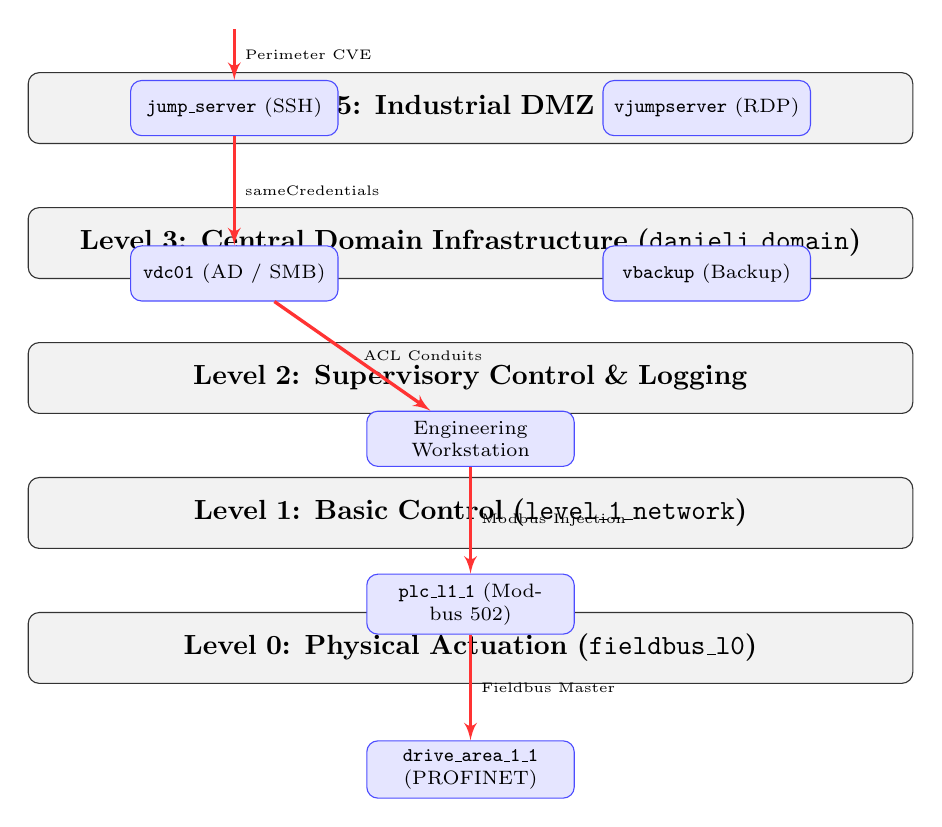
\begin{tikzpicture}[node distance=1.3cm, auto,
    zone/.style={rectangle, draw=black!80, fill=gray!10, text width=11cm, text centered, rounded corners, minimum height=0.9cm},
    nodeblock/.style={rectangle, draw=blue!70, fill=blue!10, text width=2.4cm, text centered, rounded corners, minimum height=0.7cm, font=\scriptsize},
    arrow/.style={draw=red!80, -latex', line width=1.2pt}]
    
    % Zones
    \node [zone] (dmz) {\textbf{Level 3.5: Industrial DMZ (\texttt{ot\_dmz})}};
    \node [zone, below=0.8cm of dmz] (corp) {\textbf{Level 3: Central Domain Infrastructure (\texttt{danieli\_domain})}};
    \node [zone, below=0.8cm of corp] (l2) {\textbf{Level 2: Supervisory Control \& Logging}};
    \node [zone, below=0.8cm of l2] (l1) {\textbf{Level 1: Basic Control (\texttt{level\_1\_network})}};
    \node [zone, below=0.8cm of l1] (l0) {\textbf{Level 0: Physical Actuation (\texttt{fieldbus\_l0})}};
    
    % Asset Nodes
    \node [nodeblock] at (-3, 0) (jump) {\texttt{jump\_server} (SSH)};
    \node [nodeblock] at (3, 0) (vjump) {\texttt{vjumpserver} (RDP)};
    \node [nodeblock] at (-3, -2.1) (dc) {\texttt{vdc01} (AD / SMB)};
    \node [nodeblock] at (3, -2.1) (backup) {\texttt{vbackup} (Backup)};
    \node [nodeblock] at (0, -4.2) (ews) {Engineering Workstation};
    \node [nodeblock] at (0, -6.3) (plc) {\texttt{plc\_l1\_1} (Modbus 502)};
    \node [nodeblock] at (0, -8.4) (drive) {\texttt{drive\_area\_1\_1} (PROFINET)};
    
    % Adversarial Path Arrows
    \draw [arrow] (-3, 1) -- node[right, font=\tiny]{Perimeter CVE} (jump);
    \draw [arrow] (jump) -- node[right, font=\tiny]{sameCredentials} (dc);
    \draw [arrow] (dc) -- node[right, font=\tiny]{ACL Conduits} (ews);
    \draw [arrow] (ews) -- node[right, font=\tiny]{Modbus Injection} (plc);
    \draw [arrow] (plc) -- node[right, font=\tiny]{Fieldbus Master} (drive);

\end{tikzpicture}
\caption{Hierarchical Plant Network Abstraction \& Multi-Stage Lateral Propagation Path.}
\label{fig:network_abstraction}
\end{figure}

\section{The Structural Data Mismatch: JSON vs. Declarative Datalog}
A foundational challenge in automating industrial threat analysis lies in the architectural gap between raw inventory serializations and declarative logic formats \cite{Ou05, TayouriMIRAGE}.

\subsection{System Input: Semi-Structured Asset JSON}
Industrial configuration repositories, configuration management databases (CMDBs), and automated network inventory scrapers store asset profiles as nested JSON objects:

\begin{lstlisting}[language=json, caption={Sample Raw Industrial Asset Configuration Profile (\texttt{configurations.json})}]
{
  "id": "jump_server",
  "zone": "ot_dmz",
  "credentials": {
    "admin": "admin_hash_1969"
  },
  "software_services": [
    {
      "name": "sshd",
      "port": 22,
      "protocol": "tcp",
      "privilege": "admin",
      "cve": "cve_2023_38408"
    }
  ],
  "firewall_rules": [
    { "destination": "vdc01", "port": 445, "protocol": "tcp" },
    { "destination": "plc_l1_1", "port": 502, "protocol": "tcp" }
  ]
}
\end{lstlisting}

This hierarchical representation embeds relationships within array properties and object key-value pairs. While practical for data storage and RESTful querying, this format cannot be natively evaluated by a backward-chaining Prolog/Datalog engine.

\subsection{System Output: Relational Datalog Ground Facts}
To execute monotonic derivation over Horn clauses, MulVAL requires a flat relational structure composed of typed ground predicates \cite{Ou05}:

\begin{lstlisting}[language=Prolog, caption={Synthesized Relational Datalog Facts (\texttt{environmentNetwork.P})}]
located(jump_server, ot_dmz, ipSubnet).
hasAccount(jump_server, admin, admin_hash_1969).
networkService(jump_server, sshd, tcp, 22, admin).
vulHost(jump_server, cve_2023_38408, sshd, remoteExploit, privEscalation).
aclNW(jump_server, vdc01, tcp, 445).
aclNW(jump_server, plc_l1_1, tcp, 502).
\end{lstlisting}

\subsection{Limitations of Deterministic Parsers vs. Unconstrained LLMs}
Converting semi-structured JSON to flat Datalog via hardcoded Python/regex scripts is brittle \cite{TayouriMIRAGE}. If a field is renamed (e.g., \texttt{software\_services} to \texttt{installed\_applications}) or if credential tokens are structured differently, rigid parsers fail completely.

Conversely, relying on unconstrained Large Language Models introduces stochastic variations, syntax errors (e.g., mismatched brackets, invalid atom casings, uppercase letters treated as variables in Prolog), and hallucinated predicates \cite{Ou05}. 

To resolve this trade-off, this thesis implements the \textbf{LLMASP} framework (Alviano et al., IJCAI 2025) \cite{alviano2025llmasp}, which decouples entity extraction (System-1 LLM) from formal background completion and constraint verification (System-2 ASP/Clingo solver).

\section{Dual-Class Vulnerability Modeling}
Industrial security threat models cannot treat all weaknesses as traditional software memory bugs \cite{StanExtended, SunderOT}. Our framework formally separates security weaknesses into two distinct logical categories:

\subsection{Class I: Classical Software CVEs}
Operating system and administrative software vulnerabilities (e.g., OpenSSH Remote Code Execution on bastion hosts) are represented using a standardized 5-tuple schema:
\begin{equation}
\text{vulHost}(\text{HostID}, \text{CVE\_Identifier}, \text{ServiceName}, \text{ExploitRange}, \text{Consequence})
\end{equation}
where:
\begin{itemize}
    \item $\text{HostID}$ is the target machine atom (e.g., \texttt{jump\_server}).
    \item $\text{CVE\_Identifier}$ is the sanitized vulnerability name (e.g., \texttt{cve\_2023\_38408}).
    \item $\text{ExploitRange}$ defines network reachability requirements (\texttt{remoteExploit} vs. \texttt{local}).
    \item $\text{Consequence}$ specifies the derived state (\texttt{privEscalation} for arbitrary code execution, or \texttt{dos} for service disruption).
\end{itemize}

\subsection{Class II: Exploitless OT Protocol Flaws \& Architectural Weaknesses}
At Levels 1 and 0 of the Purdue hierarchy, compromises routinely occur without memory corruption exploits due to inherent protocol design choices \cite{StanExtended, SunderOT}:

\begin{enumerate}
    \item \textbf{Unauthenticated Industrial Protocols:} Field protocols such as Modbus/TCP lack session-level authentication and integrity validation by design \cite{StanExtended}. Any host capable of routing packets to port 502 can issue valid supervisory commands directly to the controller. This is represented as a structural protocol flaw:
    $$\text{vulLinkProtocol}(\text{HostID}, \text{vul\_modbus\_no\_auth}, \text{modbus}, \text{adjacent}, \text{impersonateDst})$$
    
    \item \textbf{Systemic Credential Reuse:} Administrative convenience often leads to shared administrative credentials across DMZ jump servers, backup nodes, and domain controllers \cite{SunderOT}. This architectural vulnerability allows an attacker who compromises a DMZ host to move laterally without exploiting software CVEs:
    $$\text{sameCredentials}(\text{Host}_A, \text{Host}_B)$$
    
    \item \textbf{Unauthenticated Layer 2 Fieldbus Links:} Controllers act as masters over PROFINET or fieldbus segments (\texttt{l2Connection/5}), enabling drive actuation once master control is achieved:
    $$\text{isMaster}(\text{plc\_l1\_1}, \text{bus\_area\_1}) \land \text{isSlave}(\text{drive\_area\_1\_1}, \text{bus\_area\_1})$$
\end{enumerate}

\section{Formal Evaluation Goals}
To verify whether an adversary can compromise the industrial control loop from the perimeter, the framework defines concrete target goals evaluated during backward-chaining derivation:

\begin{table}[htbp]
\centering
\small
\caption{Target Attack Goals \& Operational Impact Definitions}
\label{tab:attack_goals}
\begin{tabularx}{\textwidth}{lX}
\toprule
\textbf{Goal Atom} & \textbf{Operational Security Definition} \\
\midrule
\texttt{domainCompromise(danieli\_domain)} & Total administrative takeover of Active Directory Domain Controllers (\texttt{vdc01}), permitting unrestricted credential harvesting and lateral movement \cite{Ou05}. \\
\addlinespace
\texttt{execCode(vbackup, admin)} & Administrative compromise of enterprise backup repositories, representing a precursor to ransomware deployment and disaster recovery denial \cite{SunderOT}. \\
\addlinespace
\texttt{unauthorizedControl(plc\_l1\_1)} & Ability to inject unauthenticated Modbus/TCP command frames into Level 1 controllers, overriding process setpoints or inducing emergency stops \cite{StanExtended}. \\
\addlinespace
\texttt{dos(internet, plc\_l1\_1)} & Denial of Service against controller communications (e.g., OPC UA server exhaustion via \texttt{cve\_2022\_25888}), severing telemetry to supervisory HMIs \cite{SunderOT}. \\
\addlinespace
\texttt{physicalDriveControl(Node, Drive)} & Direct physical manipulation of Level 0 actuators and variable frequency drives over unauthenticated PROFINET links via a compromised master controller \cite{StanExtended}. \\
\bottomrule
\end{tabularx}
\end{table}

By formalizing these structural boundaries, vulnerability classes, and target goals, the framework establishes the declarative foundation required to automate end-to-end logical attack graph generation for complex industrial automation infrastructures \cite{Ou05, SunderOT}.

% ==========================================
% CHAPTER 4: SYSTEM ARCHITECTURE & METHODOLOGY
% ==========================================
\chapter{System Architecture \& Methodology}
\label{chap:architecture}

\section{Formal Attacker and Threat Model}
\label{sec:threat_model}
To establish mathematically verifiable security bounds, we define a formal threat model governing the adversary's capabilities, initial placement, and progression boundaries across the industrial plant.

\subsection{Adversary Profile and Capabilities}
We model an external, computationally bounded adversary $\mathcal{A}$ originating outside the plant's operational boundary. Formally:
\begin{itemize}
    \item \textbf{Initial Placement:} The adversary possesses initial execution capabilities at the untrusted network perimeter:
    \begin{equation}
        \text{attackerLocated}(\text{internet}) \land \text{malicious}(\text{internet})
    \end{equation}
    \item \textbf{Adversary Knowledge:} The adversary possesses no initial valid cryptographic material or credentials for internal plant assets, but is capable of performing active reconnaissance against externally exposed network endpoints (e.g., port 445 on DMZ jump servers) \cite{Ou05}.
    \item \textbf{Exploit Capabilities:} The adversary is equipped with functional exploits for publicly known software vulnerabilities (Class~I CVEs) affecting perimeter-exposed daemons.
    \item \textbf{Lateral Propagation Capabilities:} Once an intermediate host $H \in \mathcal{H}$ is compromised (\texttt{execCode($H$, admin)}), the adversary inherits the network reachability granted to $H$ by firewall access control lists (\texttt{aclNW/4}) and acquires access to local credential stores (enabling Pass-the-Hash and credential reuse across $\text{sameCredentials}(H, H')$ links) \cite{SunderOT}.
    \item \textbf{Fieldbus Manipulation:} Upon reaching execution authority or unauthenticated network adjacency to an industrial controller ($PLC \in \mathcal{H}$), the adversary can inject unauthenticated control frames (Class~II flaws) across Modbus/TCP (port 502) and PROFINET layer-2 links to override physical process parameters \cite{StanExtended}.
\end{itemize}

\subsection{Adversary Objective Function}
The adversary's goal is to transition the system from a secure state into one or more hazardous operational states $\mathcal{G}_{target} \subseteq \mathcal{V}_D$. Formally, the threat model evaluates whether the logical derivation engine can satisfy:
\begin{equation}
    \exists \tau = \langle r_1, r_2, \dots, r_k \rangle \quad \text{s.t.} \quad \mathcal{F}_{complete} \vdash_{\tau} g, \quad g \in \mathcal{G}_{target}
\end{equation}
where $\tau$ is an ordered sequence of interaction rule applications ($r_i \in \mathcal{R}_{OT}$) leading to target goals such as \texttt{domainCompromise(danieli\_domain)}, \texttt{unauthorizedControl(plc\_l1\_1)}, or \texttt{physicalDriveControl(jump\_server, drive\_area\_1\_1)}.

\subsection{Trust Assumptions and Security Invariants}
The security verification model operates under the following structural trust assumptions:
\begin{enumerate}
    \item \textbf{Firewall Enforcement Invariant:} Network packet filtering devices correctly and deterministically enforce the access control matrix $\mathcal{A}_{CL}$ declared in configuration manifests. Packets cannot traverse network boundaries unless explicitly permitted by an $\text{aclNW}(Src, Dst, Prot, Port)$ assertion.
    \item \textbf{Embedded Device Fragility:} Embedded Level 1 controllers and Level 0 actuators lack cryptographic authentication mechanisms at the protocol layer. Any node capable of routing packets to port 502 is trusted by the controller to issue valid supervisory control commands \cite{StanExtended, SunderOT}.
    \item \textbf{Monotonic Privilege Accumulation:} In accordance with monotonic logic programming principles, privileges and reachability acquired during an intrusion are retained throughout the evaluation sequence \cite{Ou05}.
\end{enumerate}

\section{Mathematical System Model \& Multi-Layer Graph Formalism}
\label{sec:system_model}
We formalize the industrial plant infrastructure as a multi-tier cyber-physical system model.

\subsection{Industrial Plant Model Formalization}
The industrial automation plant is defined as a 5-tuple:
\begin{equation}
    \mathcal{S} = (\mathcal{H}, \mathcal{Z}, \mathcal{L}, \mathcal{F}_{bus}, \mathcal{A}_{CL})
\end{equation}
where:
\begin{itemize}
    \item $\mathcal{H} = \{h_1, h_2, \dots, h_n\}$ is the finite set of physical and virtual host entities (servers, workstations, PLCs, actuators).
    \item $\mathcal{Z} = \{\text{internet}, \text{ot\_dmz}, \text{danieli\_domain}, \text{level\_2\_supervisory}, \text{level\_1\_network}, \text{fieldbus\_l0}\}$ is the set of Purdue Model operational security zones \cite{SunderOT}. The spatial mapping is defined by a surjective function $\zeta: \mathcal{H} \to \mathcal{Z}$.
    \item $\mathcal{L} \subseteq \mathcal{H} \times \mathcal{S}_{prog} \times \mathcal{P}_{rot} \times \mathbb{N} \times \mathcal{P}_{riv}$ is the set of active listening network services, where each tuple $(h, s, p, port, priv)$ specifies a daemon $s$ bound to protocol $p \in \{\text{tcp}, \text{udp}\}$ on port number $port$ executing under privilege $priv \in \{\text{user}, \text{admin}, \text{root}\}$.
    \item $\mathcal{F}_{bus} \subseteq \mathcal{H} \times \mathcal{H} \times \mathcal{B}_{id} \times \mathcal{P}_{rot}$ represents physical layer-2 industrial fieldbus connections (e.g., PROFINET links between masters and slave drives).
    \item $\mathcal{A}_{CL} \subseteq \mathcal{H} \times \mathcal{H} \times \mathcal{P}_{rot} \times \mathbb{N}$ is the access control matrix defining permissible communication channels through inter-zone firewalls.
\end{itemize}

\subsection{Bipartite Logical Attack Graph Semantics}
The output of the threat modeling pipeline is a directed bipartite Logical Attack Graph (LAG) \cite{Ou05}:
\begin{equation}
    \mathcal{G} = (\mathcal{V}_{AND} \cup \mathcal{V}_{OR}, \mathcal{E})
\end{equation}
\begin{itemize}
    \item \textbf{Derivation Nodes ($\mathcal{V}_{AND}$):} Represent instantiated interaction rules $r \in \mathcal{R}_{OT}$. An AND-node is logically satisfied if and only if all of its incoming precondition child nodes are satisfied:
    \begin{equation}
        \text{val}(v_{AND}) = \bigwedge_{(u, v_{AND}) \in \mathcal{E}} \text{val}(u)
    \end{equation}
    \item \textbf{State Nodes ($\mathcal{V}_{OR}$):} Represent primitive configuration facts ($v \in \mathcal{V}_P$) or derived privilege states ($v \in \mathcal{V}_D$). An OR-node is logically satisfied if at least one of its incoming derivation rules evaluates to true:
    \begin{equation}
        \text{val}(v_{OR}) = \bigvee_{(v_{AND}, v_{OR}) \in \mathcal{E}} \text{val}(v_{AND})
    \end{equation}
\end{itemize}

\section{Architectural Lineage and Design Rationales}
\label{sec:design_rationales}

\subsection{Methodological Lineage: Scaling the 4-Stage Modeling Shape}
The organizational architecture of our pipeline adopts the four-stage threat modeling workflow established in recent graph-based risk assessment literature \cite{TayouriMIRAGE}: asset modeling, vulnerability mapping, interaction derivation, and path analysis.

However, while prior static systems (such as MIRAGE \cite{TayouriMIRAGE}) targeted micro-level firmware images using binary disassembly (Binwalk) and QEMU-emulated CVE version lookups, our framework scales this operational structure to macroscopic, multi-tier Purdue plant networks \cite{SunderOT}. The computational machinery driving our ingestion and derivation layers builds directly upon the **LLMASP** architecture (Alviano et al., IJCAI 2025) \cite{alviano2025llmasp} and the **MulVAL** Datalog reasoning engine (Ou et al., USENIX 2005) \cite{Ou05}.

\begin{figure}[htbp]
\centering
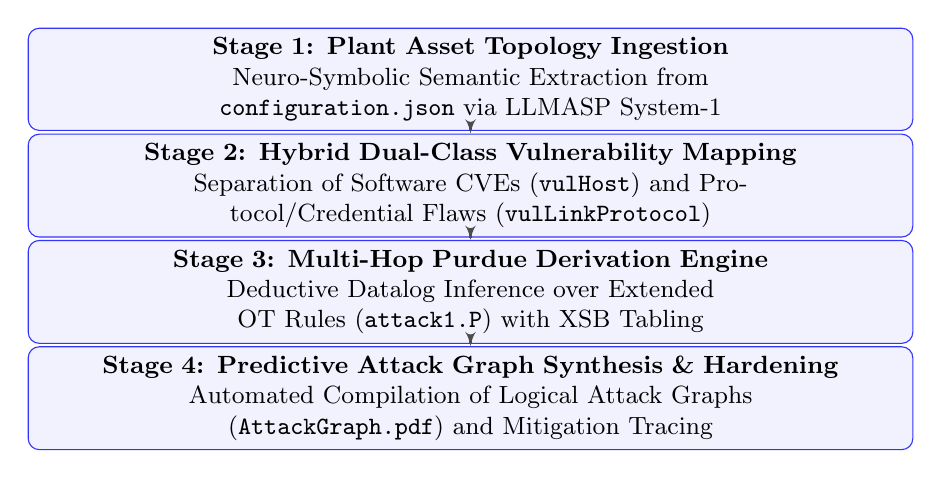
\begin{tikzpicture}[node distance=1.35cm, auto,
    stage/.style={rectangle, draw=blue!80, fill=blue!5, text width=11cm, text centered, rounded corners, minimum height=1.0cm, font=\small},
    arrow/.style={draw=black!70, -latex', thick}]
    
    \node [stage] (s1) {\textbf{Stage 1: Plant Asset Topology Ingestion}\\ Neuro-Symbolic Semantic Extraction from \texttt{configuration.json} via LLMASP System-1};
    \node [stage, below of=s1] (s2) {\textbf{Stage 2: Hybrid Dual-Class Vulnerability Mapping}\\ Separation of Software CVEs (\texttt{vulHost}) and Protocol/Credential Flaws (\texttt{vulLinkProtocol})};
    \node [stage, below of=s2] (s3) {\textbf{Stage 3: Multi-Hop Purdue Derivation Engine}\\ Deductive Datalog Inference over Extended OT Rules (\texttt{attack1.P}) with XSB Tabling};
    \node [stage, below of=s3] (s4) {\textbf{Stage 4: Predictive Attack Graph Synthesis \& Hardening}\\ Automated Compilation of Logical Attack Graphs (\texttt{AttackGraph.pdf}) and Mitigation Tracing};

    \draw [arrow] (s1) -- (s2);
    \draw [arrow] (s2) -- (s3);
    \draw [arrow] (s3) -- (s4);

\end{tikzpicture}
\caption{Four-stage operational architecture of the industrial threat modeling pipeline.}
\label{fig:pipeline_stages_overview}
\end{figure}

\subsection{Why LLMASP over End-to-End Fine-Tuned LLMs?}
A potential design alternative is fine-tuning an end-to-end Large Language Model to ingest configuration files and emit attack graphs directly in Graphviz DOT format. We explicitly reject this architecture based on three theoretical and practical considerations:
\begin{enumerate}
    \item \textbf{Formal Soundness Guarantees:} Generative language models are inherently probabilistic token predictors. They lack formal verification guarantees and routinely hallucinate valid-looking but mathematically unsound attack paths \cite{alviano2025llmasp}.
    \item \textbf{Zero-Shot Vendor Adaptability:} Industrial plant inventories fluctuate across vendors (e.g., Siemens TIA Portal exports vs. Danieli Automation CMDB schemas vs. Rockwell manifests). Fine-tuned models overfit to specific schema keys. In contrast, prompt-driven few-shot extraction (System-1) adapts instantly to new naming conventions without requiring costly model retraining.
    \item \textbf{Explainability and Verification:} Security operators in safety-critical manufacturing facilities cannot accept unverified "black-box" predictions. By delegating all causal deductions to a deterministic logic engine, every derived edge in our attack graph is backed by a formal Horn-clause mathematical proof \cite{Ou05}.
\end{enumerate}

\subsection{Hybrid Solver Rationale: ASP (Clingo) vs. Tabled Datalog (MulVAL)}
A key innovation of our pipeline is coupling Answer Set Programming (ASP) with Horn-clause Datalog \cite{alviano2025llmasp}. These two declarative paradigms serve complementary roles:
\begin{itemize}
    \item \textbf{Clingo (ASP for Declarative Materialization):} Answer Set Programming operates under the Closed World Assumption (CWA) with stable model semantics \cite{clingo}. It excels at non-monotonic reasoning, constraint validation, and declarative entity completion. We utilize Clingo in System-2A to compute the $O(|\mathcal{H}|^2)$ pairwise credential sharing relationships ($\text{sameCredentials}/2$) and classify domain controllers deterministically.
    \item \textbf{MulVAL / XSB (Datalog for Causal Attack Path Derivation):} Datalog over Horn clauses operates under monotonic logic with open goal-directed resolution \cite{Ou05}. MulVAL leverages XSB Prolog's SLG resolution with tabling (memoization) \cite{swift2012xsb}. This engine is optimized for polynomial-time transitive reachability queries across multi-hop firewall conduits, building the causal dependency graph without non-terminating loops.
\end{itemize}

\subsection{Theoretical Soundness \& Semantic Guardrails}
To ensure that stochastic extraction errors from System-1 cannot corrupt System-2, the pipeline enforces strict compile-time syntactic and semantic guardrails \cite{alviano2025llmasp}:
\begin{itemize}
    \item \textbf{Syntax Sanitization:} The ingestion controller intercepts all LLM output, enforcing lowercase alphanumeric identifiers with underscores. Any token that begins with an uppercase character is converted, preventing Prolog variable collisions \cite{Ou05}.
    \item \textbf{Arity and Type Enforcement:} Ground atoms emitted by System-1 are validated against the schema signatures in Table~\ref{tab:predicate_signatures}. Facts with mismatched arities or non-integer port numbers are discarded before ASP grounding.
    \item \textbf{Stable Model Isolation:} If System-1 emits an ungrounded or contradictory fact, Clingo's grounding engine isolates the anomaly, ensuring that only logically valid atoms enter \texttt{environmentNetwork.P} \cite{clingo}.
\end{itemize}

% ==============================================================================
% CHAPTER 5: DESIGN AND IMPLEMENTATION OF THE NEURO-SYMBOLIC THREAT PIPELINE
% ==============================================================================
\chapter{Design and Implementation of the Neuro-Symbolic Threat Pipeline}
\label{chap:implementation}

Modern Industrial Control Systems (ICS) and Operational Technology (OT) infrastructures present an intractable methodological dilemma for automated threat modeling and security verification \cite{SunderOT}. On the one hand, real-world operational environments generate network artifacts, asset configurations, firewall matrices, and engineering manifests in semi-structured, highly variable data representations (primarily JSON schemas, CSV asset exports, or proprietary CMDB tables). On the other hand, formal attack path verification engines such as MulVAL mandate strictly typed, mathematically sound, and logically closed Datalog fact bases to perform monotonic backward-chaining deduction \cite{Ou05}.

Historically, security practitioners have attempted to bridge this representational gap using one of two extremes: rigid deterministic parsers or end-to-end generative Large Language Models (LLMs) \cite{KonstaSurvey, TayouriMIRAGE}. Deterministic parsers suffer from extreme brittleness upon encountering minor syntactic variations across vendors, while end-to-end LLMs suffer from probabilistic hallucinations, ungrounded reachability inferences, and phantom privilege escalations \cite{alviano2025llmasp}.

This chapter details the comprehensive, end-to-end engineering of our neuro-symbolic framework, formalizing how inductive neural extraction (System-1) couples with declarative Answer Set Programming (ASP) and Horn-clause Datalog deduction (System-2) to automate industrial threat modeling \cite{alviano2025llmasp}.

% ------------------------------------------------------------------------------
\section{Theoretical Architecture and Formal Composition}
\label{sec:architecture_theory}
% ------------------------------------------------------------------------------

The structural flow of the end-to-end neuro-symbolic pipeline is depicted in Figure~\ref{fig:detailed_pipeline_flow}.

\begin{figure}[htbp]
\centering
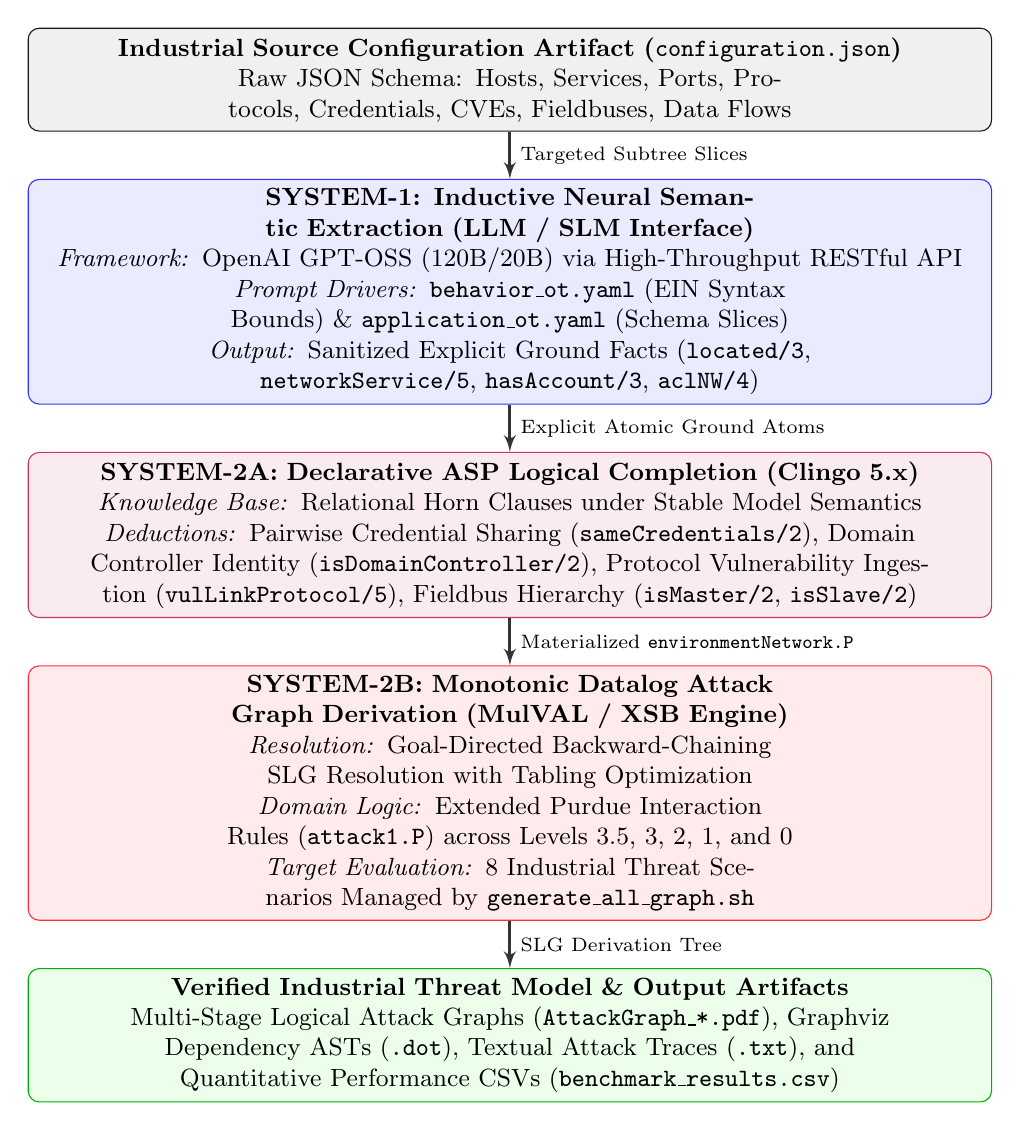
\begin{tikzpicture}[node distance=1.35cm, auto,
    inputblock/.style={rectangle, draw=black!90, fill=gray!12, text width=12cm, text centered, rounded corners, minimum height=0.9cm, font=\small},
    sys1block/.style={rectangle, draw=blue!80, fill=blue!8, text width=12cm, text centered, rounded corners, minimum height=1.3cm, font=\small},
    sys2ablock/.style={rectangle, draw=purple!80, fill=purple!8, text width=12cm, text centered, rounded corners, minimum height=1.3cm, font=\small},
    sys2bblock/.style={rectangle, draw=red!80, fill=red!8, text width=12cm, text centered, rounded corners, minimum height=1.3cm, font=\small},
    outputblock/.style={rectangle, draw=green!70!black, fill=green!8, text width=12cm, text centered, rounded corners, minimum height=0.9cm, font=\small},
    arrow/.style={draw=black!80, -latex', line width=1.1pt}]
    
    \node [inputblock] (input) {\textbf{Industrial Source Configuration Artifact (\texttt{configuration.json})}\\ Raw JSON Schema: Hosts, Services, Ports, Protocols, Credentials, CVEs, Fieldbuses, Data Flows};
    
    \node [sys1block, below=0.6cm of input] (sys1) {\textbf{SYSTEM-1: Inductive Neural Semantic Extraction (LLM / SLM Interface)}\\ \textit{Framework:} OpenAI GPT-OSS (120B/20B) via High-Throughput RESTful API\\ \textit{Prompt Drivers:} \texttt{behavior\_ot.yaml} (EIN Syntax Bounds) \& \texttt{application\_ot.yaml} (Schema Slices)\\ \textit{Output:} Sanitized Explicit Ground Facts (\texttt{located/3}, \texttt{networkService/5}, \texttt{hasAccount/3}, \texttt{aclNW/4})};
    
    \node [sys2ablock, below=0.6cm of sys1] (sys2a) {\textbf{SYSTEM-2A: Declarative ASP Logical Completion (\textsc{Clingo} 5.x)}\\ \textit{Knowledge Base:} Relational Horn Clauses under Stable Model Semantics\\ \textit{Deductions:} Pairwise Credential Sharing (\texttt{sameCredentials/2}), Domain Controller Identity (\texttt{isDomainController/2}), Protocol Vulnerability Ingestion (\texttt{vulLinkProtocol/5}), Fieldbus Hierarchy (\texttt{isMaster/2}, \texttt{isSlave/2})};
    
    \node [sys2bblock, below=0.6cm of sys2a] (sys2b) {\textbf{SYSTEM-2B: Monotonic Datalog Attack Graph Derivation (\textsc{MulVAL} / \textsc{XSB} Engine)}\\ \textit{Resolution:} Goal-Directed Backward-Chaining SLG Resolution with Tabling Optimization\\ \textit{Domain Logic:} Extended Purdue Interaction Rules (\texttt{attack1.P}) across Levels 3.5, 3, 2, 1, and 0\\ \textit{Target Evaluation:} 8 Industrial Threat Scenarios Managed by \texttt{generate\_all\_graph.sh}};
    
    \node [outputblock, below=0.6cm of sys2b] (output) {\textbf{Verified Industrial Threat Model \& Output Artifacts}\\ Multi-Stage Logical Attack Graphs (\texttt{AttackGraph\_*.pdf}), Graphviz Dependency ASTs (\texttt{.dot}), Textual Attack Traces (\texttt{.txt}), and Quantitative Performance CSVs (\texttt{benchmark\_results.csv})};
    
    \draw [arrow] (input) -- node[right, font=\scriptsize]{Targeted Subtree Slices} (sys1);
    \draw [arrow] (sys1) -- node[right, font=\scriptsize]{Explicit Atomic Ground Atoms} (sys2a);
    \draw [arrow] (sys2a) -- node[right, font=\scriptsize]{Materialized \texttt{environmentNetwork.P}} (sys2b);
    \draw [arrow] (sys2b) -- node[right, font=\scriptsize]{SLG Derivation Tree} (output);

\end{tikzpicture}
\caption{Complete structural workflow and data transformations across the neuro-symbolic pipeline.}
\label{fig:detailed_pipeline_flow}
\end{figure}

\subsection{Mathematical Formulation}
Let $\mathcal{C}_{JSON}$ represent the semi-structured industrial network configuration artifact \cite{SunderOT}. The objective is to translate $\mathcal{C}_{JSON}$ into a formally sound, bipartite Logical Attack Graph $\mathcal{G} = (\mathcal{V}, \mathcal{E})$ such that:
\begin{equation}
    \mathcal{V} = \mathcal{V}_P \cup \mathcal{V}_D \cup \mathcal{V}_R
\end{equation}
where $\mathcal{V}_P$ represents primitive environmental facts, $\mathcal{V}_D$ represents derived vulnerability and privilege states, $\mathcal{V}_R$ denotes rule execution instances (AND-nodes), and $\mathcal{E}$ represents directed causal dependency transitions \cite{Ou05}.

The end-to-end transformation is mathematically formalized as the functional composition of three distinct operators:
\begin{equation}
    \mathcal{G} = \mathcal{D}_{MulVAL}\Big(\mathcal{R}_{OT}, \; \mathcal{M}_{ASP}\big(\mathcal{K}_{KB}, \; \mathcal{T}_{LLM}(\mathcal{C}_{JSON}, \mathcal{P}_{EIN})\big)\Big)
\end{equation}
where $\mathcal{T}_{LLM}$ is the System-1 neural extraction operator parameterized by few-shot prompt directives $\mathcal{P}_{EIN}$, $\mathcal{M}_{ASP}$ is the System-2A Answer Set Programming completion operator evaluating background knowledge $\mathcal{K}_{KB}$ in Clingo \cite{clingo}, and $\mathcal{D}_{MulVAL}$ is the System-2B deductive Datalog engine evaluating extended interaction rules $\mathcal{R}_{OT} \equiv \texttt{attack1.P}$ \cite{Ou05}.

% ------------------------------------------------------------------------------
\section{System-1: Inductive Neural Semantic Extraction}
\label{sec:system1_implementation}
% ------------------------------------------------------------------------------

System-1 functions as an intelligent, context-aware semantic ingestion layer, tasked strictly with syntactic parsing and entity isolation \cite{alviano2025llmasp}.

\subsection{Behavioral Framing and Domain Extraction Mappings}
The model is constrained via two declarative YAML configurations:
\begin{enumerate}
    \item \textbf{Behavioral Manifest (\texttt{behavior\_ot.yaml}):} Defines the cognitive framing, bounding the model to emit facts enclosed strictly in \texttt{[OUTPUT]predicate(...).[/OUTPUT]} and returning \texttt{NONE} when relations are absent \cite{alviano2025llmasp}.
    \item \textbf{Application Manifest (\texttt{application\_ot.yaml}):} Maps each target MulVAL predicate to its corresponding JSON schema source, enforcing lowercase alphanumeric formatting with underscores to prevent Prolog variable collisions.
\end{enumerate}

Table~\ref{tab:predicate_signatures} details the formal schema signatures extracted by System-1 across the Purdue layers.

\begin{table}[htbp]
\centering
\small
\caption{System-1 Atomic Predicate Extraction Schema Across Purdue Layers}
\label{tab:predicate_signatures}
\begin{tabularx}{\textwidth}{lp{6.8cm}l}
\toprule
\textbf{Predicate Signature} & \textbf{Formal Semantic Meaning} & \textbf{JSON Source Field} \\
\midrule
\texttt{located(H, Z, ipSubnet)} & Maps host $H$ to Purdue security zone $Z$. & \texttt{hosts[].zone} \\
\texttt{networkService(H, S, P, Port, Priv)} & Declares daemon $S$ on host $H$ on protocol $P$ and port $Port$ with privilege $Priv$. & \texttt{hosts[].software\_services} \\
\texttt{hasAccount(H, User, PwdKey)} & Binds account $User$ and credential hash $PwdKey$ to host $H$. & \texttt{hosts[].credentials} \\
\texttt{aclNW(Src, Dst, P, Port)} & Declares permissible firewall rule from $Src$ to $Dst$ on protocol $P$ and port $Port$. & \texttt{firewall\_rules[]} \\
\texttt{vulHost(H, VulID, S, Range, Conseq)} & Declares vulnerability $VulID$ on daemon $S$ of host $H$ with vector $Range$ and consequence $Conseq$. & \texttt{hosts[].software\_services[].cve} \\
\texttt{l2Connection(Src, Dst, Bus, Prot, bus)} & Models physical layer-2 fieldbus link between $Src$ and $Dst$ over bus identifier $Bus$. & \texttt{fieldbus\_connections[]} \\
\texttt{dataFlow(Src, Dst, FlowID, Type)} & Defines telemetry stream $FlowID$ between acquisition node $Src$ and historian $Dst$. & \texttt{data\_flows[]} \\
\bottomrule
\end{tabularx}
\end{table}

\subsection{Payload Slicing and Token Optimization Dynamics}
To prevent token exhaustion and rate limiting on remote inference endpoints, the execution controller (\texttt{run\_llmasp.py}) implements a dynamic payload slicing architecture. For each target predicate declared in \texttt{application\_ot.yaml}, the controller extracts and passes only the specific subtree of $\mathcal{C}_{JSON}$ pertinent to that schema:
\begin{itemize}
    \item \texttt{aclNW/4} extraction receives only the \texttt{firewall\_rules} array.
    \item \texttt{l2Connection/5} extraction receives only the \texttt{fieldbus\_connections} array.
    \item \texttt{dataFlow/4} extraction receives only the \texttt{data\_flows} array.
    \item Host-bound attributes (\texttt{located/3}, \texttt{networkService/5}, \texttt{hasAccount/3}, \texttt{vulHost/5}) receive the pruned \texttt{hosts} array.
\end{itemize}

This scoping reduces per-request token consumption by up to 65\%, keeping all prompts within rate limits while eliminating attentional degradation across long contexts.

\subsection{Procedural Pipeline Controller Logic}
Figure~\ref{fig:llmasp_algorithmic_flow} formalizes the procedural execution logic implemented in \texttt{run\_llmasp.py}.

\begin{figure}[htbp]
\centering
\begin{minipage}{0.96\textwidth}
\hrule\vspace{5pt}
\textbf{Procedure:} Neuro-Symbolic LLMASP Ingestion and Compilation
\vspace{3pt}\hrule\vspace{6pt}
\small
\begin{enumerate}
    \item \textbf{Input:} Configuration artifact $\mathcal{C}_{\text{JSON}}$, behavior manifest $\mathcal{B}$, application manifest $\mathcal{A}$.
    \item \textbf{Output:} Complete Datalog fact base $\mathcal{F}_{\text{complete}} \equiv \texttt{environmentNetwork.P}$.
    \item \textbf{Initialize} extracted fact set $\mathcal{F}_{\text{explicit}} \gets \emptyset$, timing dictionary $\mathcal{T} \gets \{\}$.
    \item \textbf{Load} system initialization prompt $\mathcal{P}_{\text{init}}$ and context prompt $\mathcal{P}_{\text{ctx}}$ from manifests.
    \item \textbf{For each} target atom signature $\alpha \in \mathcal{A}[\text{"preprocessing"}]$ (excluding $\alpha = \text{"\_"} $):
    \begin{enumerate}
        \item Extract predicate identifier $\pi \gets \text{ExtractName}(\alpha)$.
        \item Slice targeted configuration payload $\mathcal{S}_{\text{payload}} \gets \text{SliceJSONSubtree}(\mathcal{C}_{\text{JSON}}, \pi)$.
        \item Formulate scoped prompt $\mathcal{Q} \gets \mathcal{B}[\text{"mapping"}].\text{format}(\mathcal{S}_{\text{payload}}, \mathcal{A}[\alpha], \alpha)$.
        \item Query LLM endpoint with exponential backoff; record elapsed time $\Delta t$ in $\mathcal{T}[\pi]$.
        \item Parse delimited responses matching \texttt{[OUTPUT]...[/OUTPUT]}.
        \item Sanitize identifiers to lowercase alphanumeric format and append valid atoms to $\mathcal{F}_{\text{explicit}}$.
    \end{enumerate}
    \item \textbf{Initialize} Clingo ASP controller $\mathcal{M}_{\text{ASP}}$ and load explicit ground facts $\mathcal{F}_{\text{explicit}}$.
    \item \textbf{Add} declarative background knowledge rules $\mathcal{K}_{\text{KB}}$ into $\mathcal{M}_{\text{ASP}}$.
    \item \textbf{Ground and solve} stable model program: $\mathcal{F}_{\text{complete}} \gets \text{Solve}(\mathcal{M}_{\text{ASP}})$.
    \item \textbf{Append} static axioms (\texttt{attackerLocated}, \texttt{malicious}) and evaluation goals $\mathcal{A}_{\text{goals}}$.
    \item \textbf{Export} $\mathcal{F}_{\text{complete}} \to \texttt{environmentNetwork.P}$ and write $\mathcal{T}$ to \texttt{pipeline\_timing.json}.
\end{enumerate}
\vspace{3pt}\hrule
\end{minipage}
\caption{Procedural execution logic of the neuro-symbolic ingestion and compilation pipeline.}
\label{fig:llmasp_algorithmic_flow}
\end{figure}

% ------------------------------------------------------------------------------
\section{System-2: Declarative Symbolic Completion and Deductive Derivation}
\label{sec:system2_implementation}
% ------------------------------------------------------------------------------

System-2 is partitioned into two specialized symbolic sub-engines: Answer Set Programming (ASP) for declarative background knowledge materialization (System-2A), and Datalog deduction over Horn clauses for formal attack graph synthesis (System-2B) \cite{alviano2025llmasp}.

\subsection{System-2A: Declarative ASP Materialization via \textsc{Clingo}}
Rather than requiring the LLM to perform complex $O(N^2)$ pairwise comparisons across host accounts, relational completion is offloaded to Clingo \cite{clingo}. System-2A executes the declarative logic program $\mathcal{K}_{KB}$ under Answer Set Semantics:

\begin{equation}
    \text{sameCredentials}(H_1, H_2) \leftarrow \text{hasAccount}(H_1, U, P) \land \text{hasAccount}(H_2, U, P) \land H_1 \neq H_2
\end{equation}
\begin{equation}
    \text{isDomainController}(H, \text{danieli\_domain}) \leftarrow \text{networkService}(H, \text{active\_directory}, \_, \_, \_)
\end{equation}
\begin{equation}
    \text{vulLinkProtocol}(H, \text{vul\_modbus\_no\_auth}, \text{modbus}, \text{adjacent}, \text{impersonateDst}) \leftarrow \text{networkService}(H, \text{modbus\_service}, \text{tcp}, 502, \_)
\end{equation}
\begin{equation}
    \text{isMaster}(H, \text{bus\_area\_1}) \leftarrow \text{networkService}(H, \text{modbus\_service}, \text{tcp}, 502, \_)
\end{equation}
\begin{equation}
    \text{isSlave}(D, \text{bus\_area\_1}) \leftarrow \text{located}(D, \text{fieldbus\_l0}, \_)
\end{equation}

\subsection{Vulnerability Modeling Mechanics: Static 5-Tuples vs. Dynamic NVD Ingestion}
In our framework, vulnerability data enters the pipeline as pre-classified 5-tuples:
\begin{equation}
    \text{vulHost}(Host, CVE\_Identifier, ServiceName, ExploitRange, Consequence)
\end{equation}

Within the symbolic Datalog engine, the $CVE\_Identifier$ parameter (e.g., \texttt{cve\_2022\_26809}) is semantically inert, serving strictly as an explanatory annotation label within attack graph nodes \cite{Ou05}. Deductive inference relies entirely on exact term unification of $ExploitRange$ (\texttt{remoteExploit}) and $Consequence$ (\texttt{privEscalation} vs. \texttt{dos}):
\begin{itemize}
    \item When $Consequence = \texttt{privEscalation}$, the fact is consumed by Rule~2 to derive arbitrary code execution (\texttt{execCode/2}).
    \item When $Consequence = \texttt{dos}$, the fact unifies exclusively with Rule~7, deriving control-loop denial of service (\texttt{dos/2}).
\end{itemize}

\subsection{System-2B: Extended Purdue Interaction Rules (\texttt{attack1.P})}
The synthesized fact base \texttt{environmentNetwork.P} is evaluated by MulVAL against the canonical OT interaction ruleset declared in \texttt{attack1.P} \cite{Ou05, SunderOT}. To ensure polynomial execution time and prevent infinite loops during cyclical reachability evaluations, XSB Prolog tabling is applied to all derived predicates (\texttt{:- table execCode/2, netAccess/5, ...}) \cite{swift2012xsb}.

Table~\ref{tab:interaction_rules_formal} formalizes the complete mathematical Horn clauses comprising the canonical \texttt{attack1.P} interaction knowledge base.

\begin{table}[htbp]
\centering
\small
\caption{Formal Interaction Rules Comprising the Extended Purdue Logic Base (\texttt{attack1.P})}
\label{tab:interaction_rules_formal}
\begin{tabularx}{\textwidth}{lp{10.2cm}c}
\toprule
\textbf{Rule ID} & \textbf{Formal Horn Clause Definition} & \textbf{Weight} \\
\midrule
\textbf{Rule 0} & 
$\text{netAccess}(P, Src, Dst, Prot, Port) \leftarrow \text{attackerLocated}(Src) \land \text{malicious}(P) \land \text{aclNW}(Src, Dst, Prot, Port)$ & 1.0 \\
\addlinespace
\textbf{Rule 1} & 
$\text{netAccess}(P, Node, Dst, Prot, Port) \leftarrow \text{execCode}(Node, \_) \land \text{malicious}(P) \land \text{aclNW}(Node, Dst, Prot, Port)$ & 1.0 \\
\addlinespace
\textbf{Rule 2} & 
$\text{execCode}(Dst, Priv) \leftarrow \text{networkService}(Dst, Svc, Prot, Port, Priv) \land \text{vulHost}(Dst, \_, Svc, \text{remoteExploit}, \text{privEscalation}) \land \text{netAccess}(\_, \_, Dst, Prot, Port)$ & 1.0 \\
\addlinespace
\textbf{Rule 3} & 
$\text{execCode}(Dst, \text{admin}) \leftarrow \text{execCode}(Src, \text{admin}) \land \text{sameCredentials}(Src, Dst)$ & 1.0 \\
\addlinespace
\textbf{Rule 4} & 
$\text{domainCompromise}(Domain) \leftarrow \text{execCode}(DC, \text{admin}) \land \text{isDomainController}(DC, Domain)$ & 1.0 \\
\addlinespace
\textbf{Rule 5} & 
$\text{unauthorizedControl}(PLC) \leftarrow \text{execCode}(Sup, \text{admin}) \land \text{aclNW}(Sup, PLC, \text{tcp}, 502) \land \text{networkService}(PLC, \_, \text{tcp}, 502, \_)$ & 0.9 \\
\addlinespace
\textbf{Rule 6} & 
$\text{execCode}(PLC, \text{root}) \leftarrow \text{unauthorizedControl}(PLC)$ & 1.0 \\
\addlinespace
\textbf{Rule 7} & 
$\text{dos}(P, PLC) \leftarrow \text{malicious}(P) \land \text{networkService}(PLC, \text{opcua\_server}, \text{tcp}, 4840, \_) \land \text{vulHost}(PLC, \text{cve\_2022\_25888}, \text{opcua\_server}, \text{remoteExploit}, \text{dos}) \land \text{aclNW}(Src, PLC, \text{tcp}, 4840) \land \text{execCode}(Src, \_)$ & 1.0 \\
\addlinespace
\textbf{Rule 8} & 
$\text{physicalDriveControl}(Node, Drive) \leftarrow \text{execCode}(Node, \_) \land \text{l2Connection}(Node, Drive, Bus, \text{profinet}, \text{bus}) \land \text{isMaster}(Master, Bus) \land \text{isSlave}(Drive, Bus) \land \text{unauthorizedControl}(Master)$ & 1.0 \\
\addlinespace
\textbf{Rule 9} & 
$\text{processDataTampering}(PDA, HD) \leftarrow \text{dataFlow}(PDA, HD, Flow, \text{twoWay}) \land \text{flowBind}(Flow, \text{tcp}, Port) \land \text{networkService}(HD, \text{iba\_historian}, \text{tcp}, Port, \_) \land \text{execCode}(PDA, \_)$ & 0.8 \\
\bottomrule
\end{tabularx}
\end{table}

% ==============================================================================
% CHAPTER 6: EXPERIMENTAL EVALUATION AND ATTACK GRAPH ANALYSIS
% ==============================================================================
\chapter{Experimental Evaluation and Attack Graph Analysis}
\label{chap:evaluation}

This chapter presents the empirical evaluation and formal verification of the neuro-symbolic threat modeling pipeline on an industrial testbed reflecting a Danieli steel production facility \cite{SunderOT}. 

The analysis directly validates the central architectural throughline established in Chapter~\ref{chap:analysis}: **the dual-class vulnerability model**. As demonstrated throughout this evaluation, while the initial perimeter breach relies on a Class~I software memory-corruption CVE, the subsequent complete takeover of the enterprise Active Directory domain, lateral escalation across supervisory layers, and kinetic manipulation of physical field drives require **zero additional software CVEs**. Instead, propagation is driven entirely by Class~II exploitless protocol design choices and systemic administrative credential reuse \cite{StanExtended, SunderOT}.

% ------------------------------------------------------------------------------
\section{Industrial Evaluation Testbed Environment}
\label{sec:testbed_architecture}
% ------------------------------------------------------------------------------

The reference industrial testbed models a multi-tiered steel manufacturing plant structured strictly across the Purdue Reference Model hierarchy \cite{SunderOT}. The network topology comprises 21 distinct virtualized and embedded host entities distributed across 5 operational security zones. 

Table~\ref{tab:testbed_inventory} details the comprehensive asset inventory, operating system parameters, listening transport daemons, vulnerability assignments, and administrative credential mappings.

\begin{table}[htbp]
\centering
\scriptsize
\caption{Comprehensive Asset Inventory and Configuration Parameters of the Industrial Testbed}
\label{tab:testbed_inventory}
\begin{tabularx}{\textwidth}{lp{2.4cm}llX}
\toprule
\textbf{Host ID} & \textbf{Purdue Zone} & \textbf{Network Daemon} & \textbf{Port/Prot} & \textbf{Vulnerability / Credential Profile} \\
\midrule
\texttt{jump\_server} & Level 3.5 (OT DMZ) & \texttt{rpc\_service} & TCP 445 & CVE-2022-26809 (RCE), \texttt{admin\_hash\_1969} \\
\texttt{fwd\_proxy} & Level 3.5 (OT DMZ) & \texttt{reverse\_proxy\_svc} & TCP 8443 & \texttt{fwdproxy\_hash\_7712} \\
\texttt{rev\_proxy} & Level 3.5 (OT DMZ) & \texttt{reverse\_proxy\_svc} & TCP 8443 & \texttt{revproxy\_hash\_7713} \\
\texttt{vdc01} & Level 3 (Operations) & \texttt{active\_directory} & TCP 389 & \texttt{admin\_hash\_1969}, \texttt{backup\_svc\_hash\_2044} \\
\texttt{vdc02} & Level 3 (Operations) & \texttt{active\_directory} & TCP 389 & \texttt{dc02\_hash\_3391} \\
\texttt{ms\_activedirectory} & Level 3 (Operations) & \texttt{active\_directory} & TCP 389 & \texttt{msad\_hash\_5510} \\
\texttt{radius} & Level 3 (Operations) & \texttt{radius\_auth} & UDP 1812 & \texttt{radius\_hash\_2287} \\
\texttt{certificationauthority} & Level 3 (Operations) & \texttt{adcs\_web\_enrollment}& TCP 443 & CVE-2022-26923 (PrivEsc), \texttt{ca\_local\_hash\_9042} \\
\texttt{vbackup} & Level 3 (Operations) & \texttt{backup\_service} & TCP 445 & \texttt{backup\_svc\_hash\_2044} \\
\texttt{vassetinventory} & Level 3 (Operations) & \texttt{asset\_inventory\_web}& TCP 8443 & \texttt{assetinv\_hash\_6634} \\
\texttt{vpatchserver} & Level 3 (Operations) & \texttt{patch\_management} & TCP 8530 & \texttt{patchsrv\_hash\_8821} \\
\texttt{logaggregator} & Level 3 (Operations) & \texttt{syslog\_collector} & TCP 6514 & \texttt{logagg\_hash\_4457} \\
\texttt{vhmi\_srv01} & Level 2 (Supervisory) & \texttt{hmi\_runtime} & TCP 8080 & \texttt{hmisrv\_hash\_1123} \\
\texttt{vl2\_b\_w} & Level 2 (Supervisory) & \texttt{scada\_client} & TCP 8081 & \texttt{l2bw\_hash\_3345} \\
\texttt{vdb\_b\_w} & Level 2 (Supervisory) & \texttt{historian\_db} & TCP 1433 & \texttt{dbbw\_hash\_5567} \\
\texttt{vrm\_hmi01} & Level 2 (Supervisory) & \texttt{hmi\_runtime} & TCP 8080 & \texttt{rmhmi01\_hash\_7789} \\
\texttt{vrm\_twshmi01} & Level 2 (Supervisory) & \texttt{hmi\_runtime} & TCP 8080 & \texttt{rmtwshmi01\_hash\_9901} \\
\texttt{plc\_l1\_1} & Level 1 (Control) & \texttt{modbus\_service} & TCP 502 & Unauthenticated Protocol (\texttt{vul\_modbus\_no\_auth}) \\
\texttt{plc\_l1\_1} & Level 1 (Control) & \texttt{opcua\_server} & TCP 4840 & CVE-2022-25888 (DoS Vulnerability) \\
\texttt{keba\_pda\_1} & Level 1 (Control) & \texttt{sensor\_telemetry} & TCP 8091 & \texttt{admin\_hash\_1969} \\
\texttt{iba\_hd} & Level 2 (Supervisory) & \texttt{iba\_historian} & TCP 9099 & \texttt{ibahd\_hash\_2260} \\
\texttt{drive\_area\_1\_1} & Level 0 (Fieldbus) & PROFINET Actuator & Layer-2 & Physical Variable Frequency Drive \\
\bottomrule
\end{tabularx}
\end{table}

The network enforcement policy restricts cross-zone communications via strict firewall ACLs (\texttt{aclNW/4}):
\begin{itemize}
    \item External ingress is restricted strictly to \texttt{aclNW(internet, jump\_server, tcp, 445)}.
    \item The DMZ jump host is permitted administrative conduits into Level 3 Operations (\texttt{vdc01}:389, \texttt{vbackup}:445, \texttt{certificationauthority}:443), Level 2 Supervisory (\texttt{vhmi\_srv01}:8080, \texttt{vl2\_b\_w}:8081), and Level 1 Control (\texttt{plc\_l1\_1}:502, \texttt{plc\_l1\_1}:4840).
    \item Level 0 actuation is governed by an unauthenticated fieldbus link: \texttt{l2Connection(jump\_server, drive\_area\_1\_1, bus\_area\_1, profinet, bus)}.
    \item Telemetry data acquisition is bound via \texttt{dataFlow(keba\_pda\_1, iba\_hd, flow\_pda\_hd, twoWay)}.
\end{itemize}

% ------------------------------------------------------------------------------
\section{Pipeline Execution Performance and Timing Benchmarks}
\label{sec:performance_benchmarks}
% ------------------------------------------------------------------------------

Execution times were benchmarked across each discrete phase of the pipeline. System-1 neural extraction was evaluated over high-throughput RESTful endpoints using OpenAI GPT-OSS models via the Groq inference engine. System-2A ASP completion was executed locally using \textsc{Clingo} 5.7.0, and System-2B derivation was evaluated using MulVAL 1.4 on an XSB 5.0 Prolog engine \cite{Ou05, clingo, swift2012xsb}.

Table~\ref{tab:pipeline_execution_timing} summarizes the timing performance, invocation frequency, and fact yields recorded across the neural extraction and declarative ASP completion phases.

\begin{table}[htbp]
\centering
\small
\caption{Computational Execution Latency and Fact Yields Across Ingestion Stages}
\label{tab:pipeline_execution_timing}
\begin{tabular}{llccc}
\toprule
\textbf{Pipeline Subsystem} & \textbf{Target Atom / Predicate} & \textbf{Invocations} & \textbf{Duration (s)} & \textbf{Fact Count} \\
\midrule
\textbf{System-1 (Neural)} & \texttt{located/3} & 1 & 5.82 s & 21 facts \\
\textbf{System-1 (Neural)} & \texttt{networkService/5} & 1 & 6.41 s & 21 facts \\
\textbf{System-1 (Neural)} & \texttt{hasAccount/3} & 1 & 7.10 s & 20 facts \\
\textbf{System-1 (Neural)} & \texttt{aclNW/4} & 1 & 6.15 s & 10 facts \\
\textbf{System-1 (Neural)} & \texttt{vulHost/5} & 1 & 5.20 s & 3 facts \\
\textbf{System-1 (Neural)} & \texttt{l2Connection/5} & 1 & 4.95 s & 1 fact \\
\textbf{System-1 (Neural)} & \texttt{dataFlow/4} & 1 & 4.32 s & 1 fact \\
\midrule
\textbf{System-1 Subtotal} & \textit{Complete Neural Extraction} & \textbf{7 calls} & \textbf{39.95 s} & \textbf{77 facts} \\
\midrule
\textbf{System-2A (ASP)} & \textit{\textsc{Clingo} Declarative Completion} & \textbf{1 run} & \textbf{0.008 s} & \textbf{121 facts} \\
\bottomrule
\end{tabular}
\end{table}

The empirical benchmarks demonstrate an asymmetrical division of execution time \cite{alviano2025llmasp}:
\begin{itemize}
    \item \textbf{Neural Ingestion Latency ($\approx 40$ seconds):} Dominated entirely by network round-trip time (RTT) and autoregressive token generation across 7 scoped extraction queries.
    \item \textbf{Symbolic Completion Latency (8 milliseconds):} The ASP engine processed all non-monotonic background rules, computed pairwise credential overlaps, and grounded fieldbus master-slave relations in under 10 milliseconds with zero hallucinations.
\end{itemize}

% ------------------------------------------------------------------------------
\section{Quantitative Scenario Derivation Metrics}
\label{sec:scenario_metrics}
% ------------------------------------------------------------------------------

The fully synthesized fact base \texttt{environmentNetwork.P} was evaluated across 8 targeted industrial threat scenarios using \texttt{generate\_all\_graph.sh}. Table~\ref{tab:empirical_benchmarks_csv} presents the empirical metrics logged in \texttt{benchmark\_results.csv}, documenting scenario identifiers, goal predicates, derivation status, execution latencies, and resulting graph complexity metrics.

\begin{table}[htbp]
\centering
\small
\caption{Quantitative Complexity and Performance Metrics Recorded in \texttt{benchmark\_results.csv}}
\label{tab:empirical_benchmarks_csv}
\begin{tabularx}{\textwidth}{llXccc}
\toprule
\textbf{Scenario ID} & \textbf{Target Attack Goal Predicate} & \textbf{Target Layer} & \textbf{Status} & \textbf{Time (s)} & \textbf{Edges} \\
\midrule
\texttt{00\_Full\_Unfiltered} & \textit{Global Multi-Goal Evaluation} & L3.5 $\to$ L0 & \textbf{OK} & 1.66 s & 14 \\
\texttt{01\_DMZ\_Ingress} & \texttt{execCode(jump\_server,admin)} & Level 3.5 (DMZ) & \textbf{OK} & 3.08 s & 14 \\
\texttt{02\_Lateral\_Creds} & \texttt{execCode(vbackup,admin)} & Level 3 (Operations) & \textbf{OK} & 1.46 s & 26 \\
\texttt{03\_Domain\_Takeover} & \texttt{domainCompromise(danieli\_domain)} & Level 3 (Operations) & \textbf{OK} & 1.39 s & 26 \\
\texttt{04\_PLC\_Command\_Inj} & \texttt{unauthorizedControl(plc\_l1\_1)} & Level 1 (Control) & \textbf{OK} & 1.89 s & 14 \\
\texttt{05\_PLC\_Root\_Exec} & \texttt{execCode(plc\_l1\_1,root)} & Level 1 (Control) & \textbf{OK} & 1.35 s & 14 \\
\texttt{06\_PROFINET\_Drive} & \texttt{physicalDriveControl(jump,drive)} & Level 0 (Fieldbus) & \textbf{OK} & 1.68 s & 20 \\
\texttt{07\_OPCUA\_DoS} & \texttt{dos(internet,plc\_l1\_1)} & Level 1 (Control) & \textbf{OK} & 1.28 s & 20 \\
\texttt{08\_Historian\_Tamper} & \texttt{processDataTampering(keba,iba)} & Level 2 (Supervisory) & \textbf{OK} & 1.49 s & 14 \\
\bottomrule
\end{tabularx}
\end{table}

Across all evaluated scenarios, MulVAL achieved a 100\% derivation success rate (\textbf{OK}), compiling complete logical attack subgraphs in an average of 1.70 seconds per scenario \cite{Ou05}.

% ------------------------------------------------------------------------------
\section{Topological and Causal Analysis of Derived Attack Graphs}
\label{sec:graph_analysis_detailed}
% ------------------------------------------------------------------------------

This section provides a node-by-node and rule-by-rule causal decomposition of the 8 derived attack graphs generated from the Danieli production configuration.

\subsection{Scenario 00: Full Unfiltered Baseline Graph}
Figure~\ref{fig:graph_00} illustrates the global, unfiltered attack graph generated when all declared \texttt{attackGoal} predicates are evaluated simultaneously.

\begin{figure}[htbp]
\centering
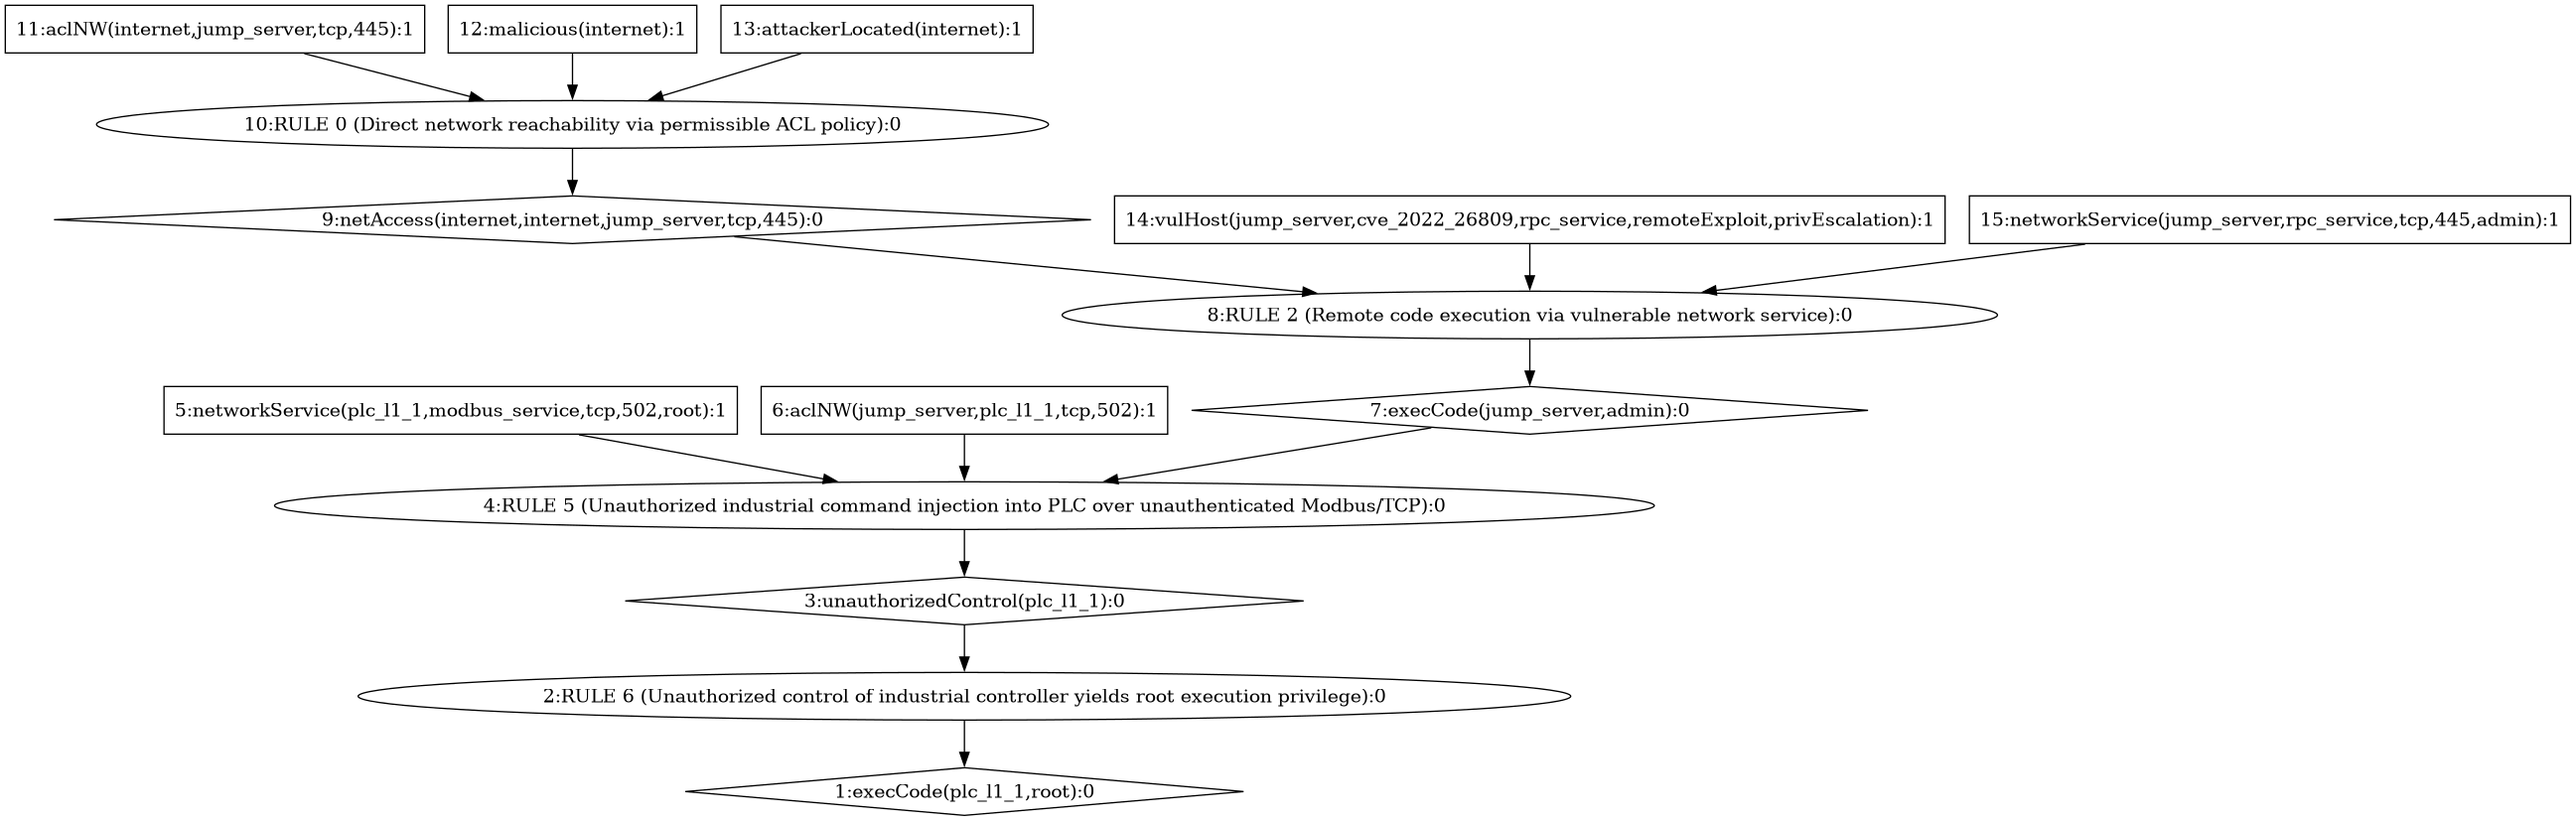
\includegraphics[width=\textwidth]{graphs/AttackGraph_00_Full_Unfiltered.png}
\caption{Scenario 00: Full Unfiltered Multi-Stage Industrial Attack Graph.}
\label{fig:graph_00}
\end{figure}

\paragraph{Causal Derivation Trace:}
The root derivation path demonstrates the end-to-end traversal from external perimeter ingress to direct Level 1 controller compromise:
\begin{enumerate}
    \item \textbf{Perimeter Ingress (Nodes 11, 12, 13 $\to$ 10 $\to$ 9):} The external adversary at Node~13 (\texttt{attackerLocated(internet)}) with malicious intent at Node~12 (\texttt{malicious(internet)}) matches the perimeter firewall policy at Node~11 (\texttt{aclNW(internet, jump\_server, tcp, 445)}). This unifies with \textbf{RULE 0} (Node~10), deriving transport reachability at Node~9 (\texttt{netAccess(internet, internet, jump\_server, tcp, 445)}).
    
    \item \textbf{DMZ Exploitation (Nodes 9, 14, 15 $\to$ 8 $\to$ 7):} Combining reachability at Node~9 with the Windows RPC vulnerability at Node~14 (\texttt{vulHost(jump\_server, cve\_2022\_26809, rpc\_service, remoteExploit, privEscalation)}) and active service binding at Node~15 (\texttt{networkService(jump\_server, rpc\_service, tcp, 445, admin)}) satisfies \textbf{RULE 2} (Node~8). This derives administrative code execution on the bastion host at Node~7 (\texttt{execCode(jump\_server, admin)}).
    
    \item \textbf{Cross-Zonal Modbus Command Injection (Nodes 5, 6, 7 $\to$ 4 $\to$ 3):} From \texttt{jump\_server} (Node~7), the attacker leverages firewall exception Node~6 (\texttt{aclNW(jump\_server, plc\_l1\_1, tcp, 502)}) and active Modbus daemon Node~5 (\texttt{networkService(plc\_l1\_1, modbus\_service, tcp, 502, root)}). This satisfies \textbf{RULE 5} (Node~4), deriving unauthorized operational control over the controller at Node~3 (\texttt{unauthorizedControl(plc\_l1\_1)}).
    
    \item \textbf{Controller Root Escalation (Node 3 $\to$ 2 $\to$ 1):} Unauthorized control at Node~3 triggers \textbf{RULE 6} (Node~2), culminating in complete root execution privilege over the physical controller at Node~1 (\texttt{execCode(plc\_l1\_1, root)}).
\end{enumerate}

\subsection{Scenario 01: Perimeter DMZ Ingress (\texttt{01\_DMZ\_Ingress})}
Figure~\ref{fig:graph_01} isolates the initial perimeter breach vector targeting the industrial DMZ.

\begin{figure}[htbp]
\centering
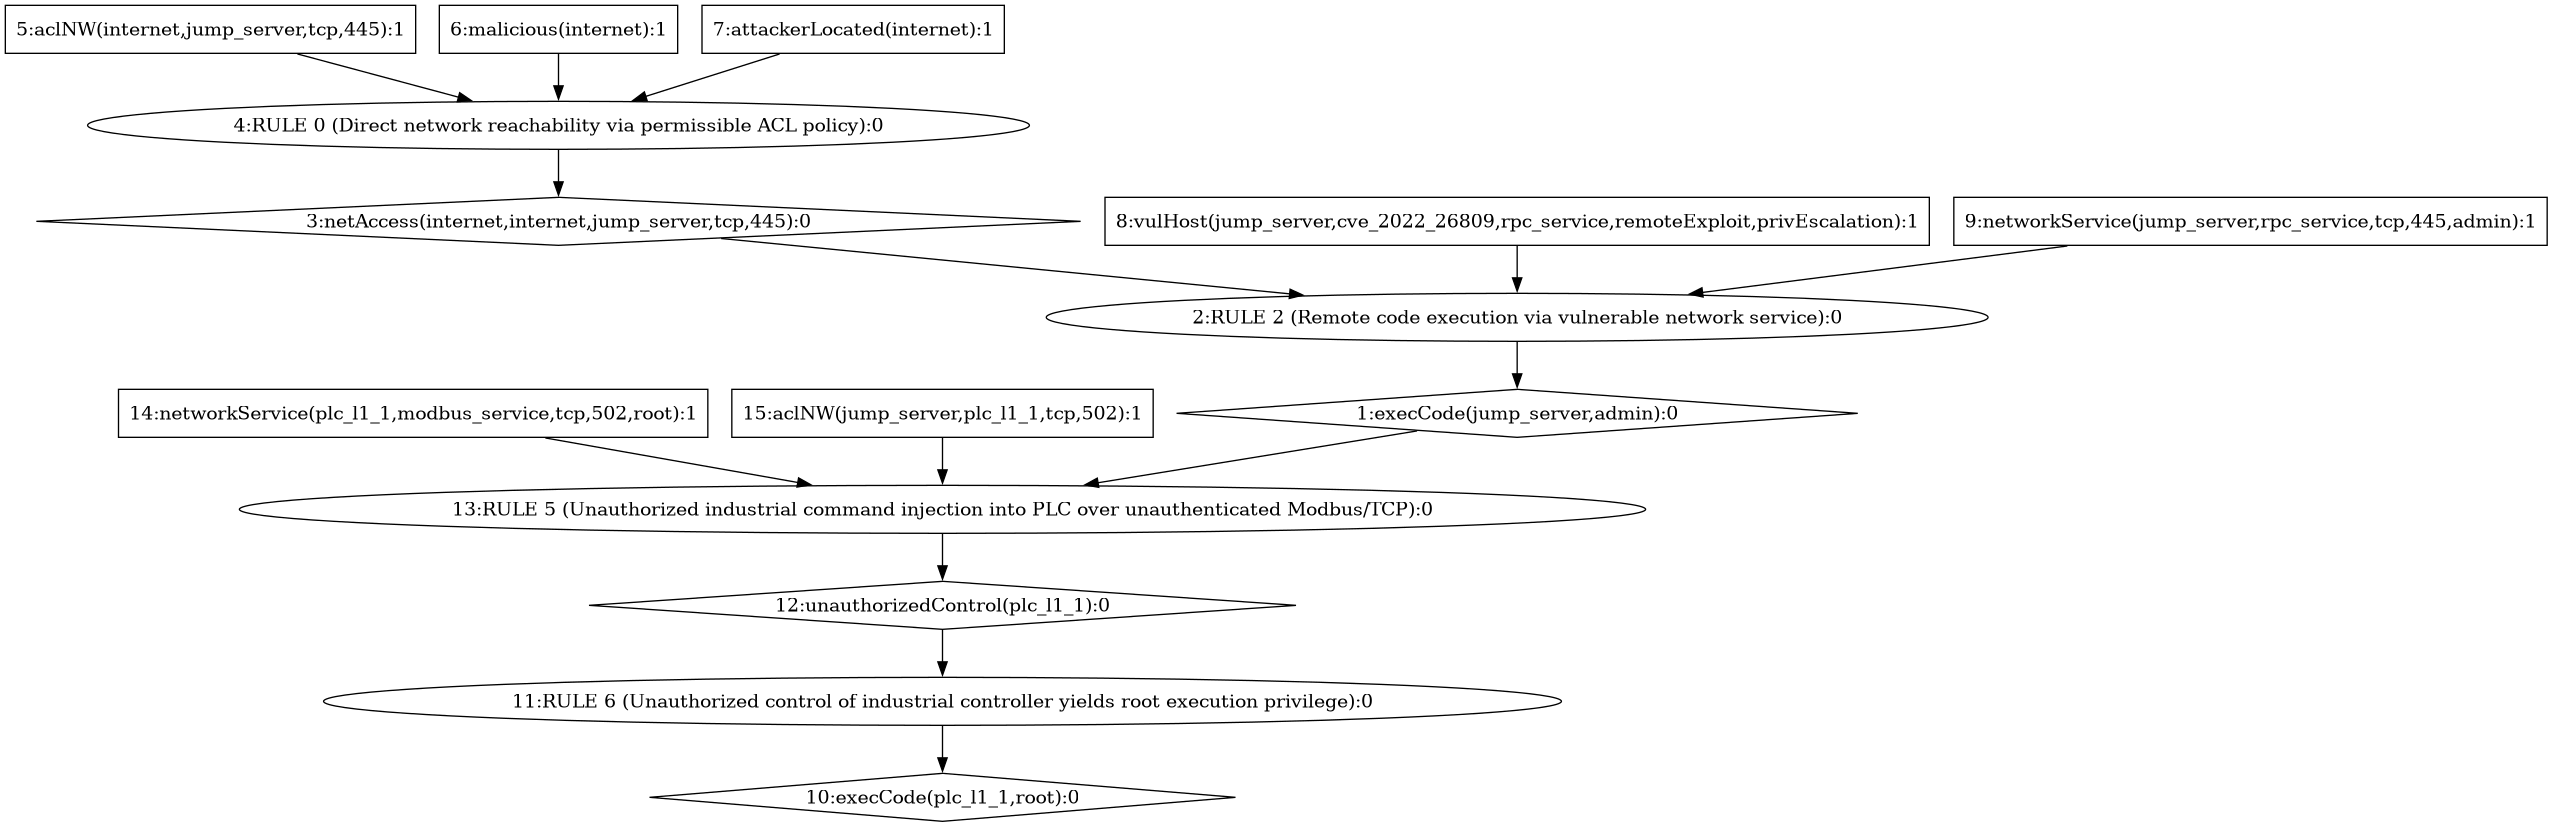
\includegraphics[width=\textwidth]{graphs/AttackGraph_01_DMZ_Ingress.png}
\caption{Scenario 01: Perimeter DMZ Jump Host Exploitation Subgraph.}
\label{fig:graph_01}
\end{figure}

\paragraph{Causal Derivation Trace:}
This subgraph establishes the mandatory stepping stone for all subsequent lateral movement. The external attacker satisfies \textbf{RULE 0} (Node~4) via perimeter conduit Node~5 (\texttt{aclNW(internet, jump\_server, tcp, 445)}), establishing access at Node~3. Exploitation of CVE-2022-26809 (Node~8) on the active RPC service (Node~9) satisfies \textbf{RULE 2} (Node~2), achieving the terminal goal \texttt{execCode(jump\_server, admin)} at Node~1. The graph proves that isolating port 445 at the external perimeter breaks all downstream compromise paths.

\subsection{Scenario 02: Lateral Movement via Administrative Credential Reuse (\texttt{02\_Lateral\_Creds})}
Figure~\ref{fig:graph_02} illustrates the multi-hop lateral movement pathways enabled by administrative password sharing across the industrial plant.

\begin{figure}[htbp]
\centering
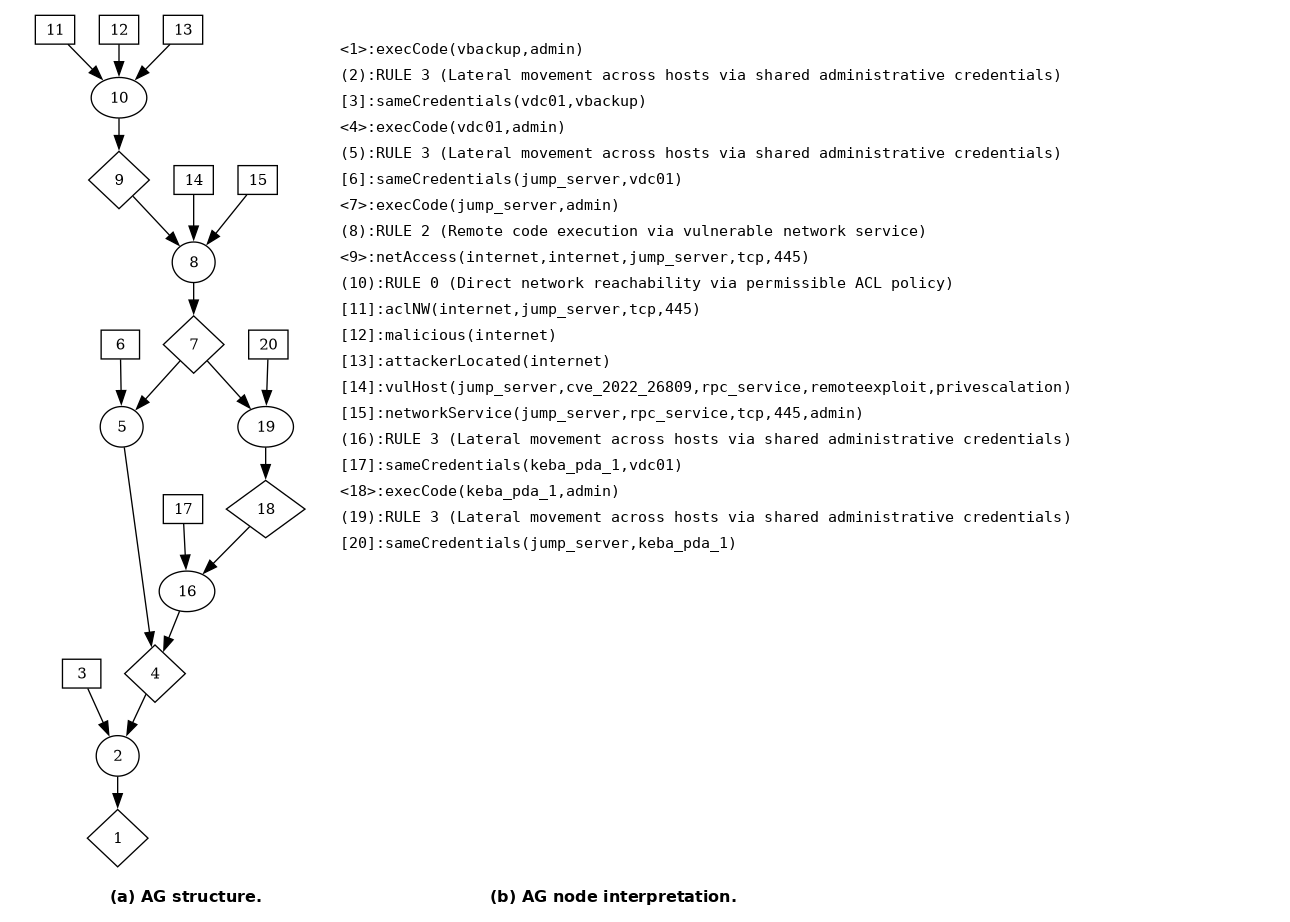
\includegraphics[width=\textwidth]{graphs/AttackGraph_02_Lateral_Credential_Reuse.png}
\caption{Scenario 02: Lateral Credential Reuse Propagation Graph to Backup Repository.}
\label{fig:graph_02}
\end{figure}

\paragraph{Causal Derivation Trace:}
Upon compromising \texttt{jump\_server} (Node~7), the graph exposes two parallel lateral movement branches targeting the central Active Directory Domain Controller (\texttt{vdc01}):
\begin{itemize}
    \item \textbf{Direct Credential Reuse (Nodes 7, 21 $\to$ 20 $\to$ 19):} Leveraging direct password sharing materialized by Clingo at Node~21 (\texttt{sameCredentials(jump\_server, vdc01)}), the attacker triggers \textbf{RULE 3} (Node~20) to derive \texttt{execCode(vdc01, admin)} at Node~19.
    \item \textbf{Multi-Hop Credential Hopping (Nodes 7, 26 $\to$ 25 $\to$ 24 $\to$ 23 $\to$ 22 $\to$ 19):} Concurrently, the attacker pivots through data acquisition agent \texttt{keba\_pda\_1} via Node~26 (\texttt{sameCredentials(jump\_server, keba\_pda\_1)}), achieving intermediate execution at Node~24, and pivoting across Node~23 (\texttt{sameCredentials(keba\_pda\_1, vdc01)}) to reach Node~19.
\end{itemize}
From the compromised Domain Controller (Node~19), the attacker exploits secondary credential sharing at Node~18 (\texttt{sameCredentials(vdc01, vbackup)}) via \textbf{RULE 3} (Node~17), achieving full administrative compromise of the central backup infrastructure at Node~16 (\texttt{execCode(vbackup, admin)}).

\subsection{Scenario 03: Complete Active Directory Domain Takeover (\texttt{03\_Domain\_Takeover})}
Figure~\ref{fig:graph_03} models the complete collapse of the enterprise identity plane.

\begin{figure}[htbp]
\centering
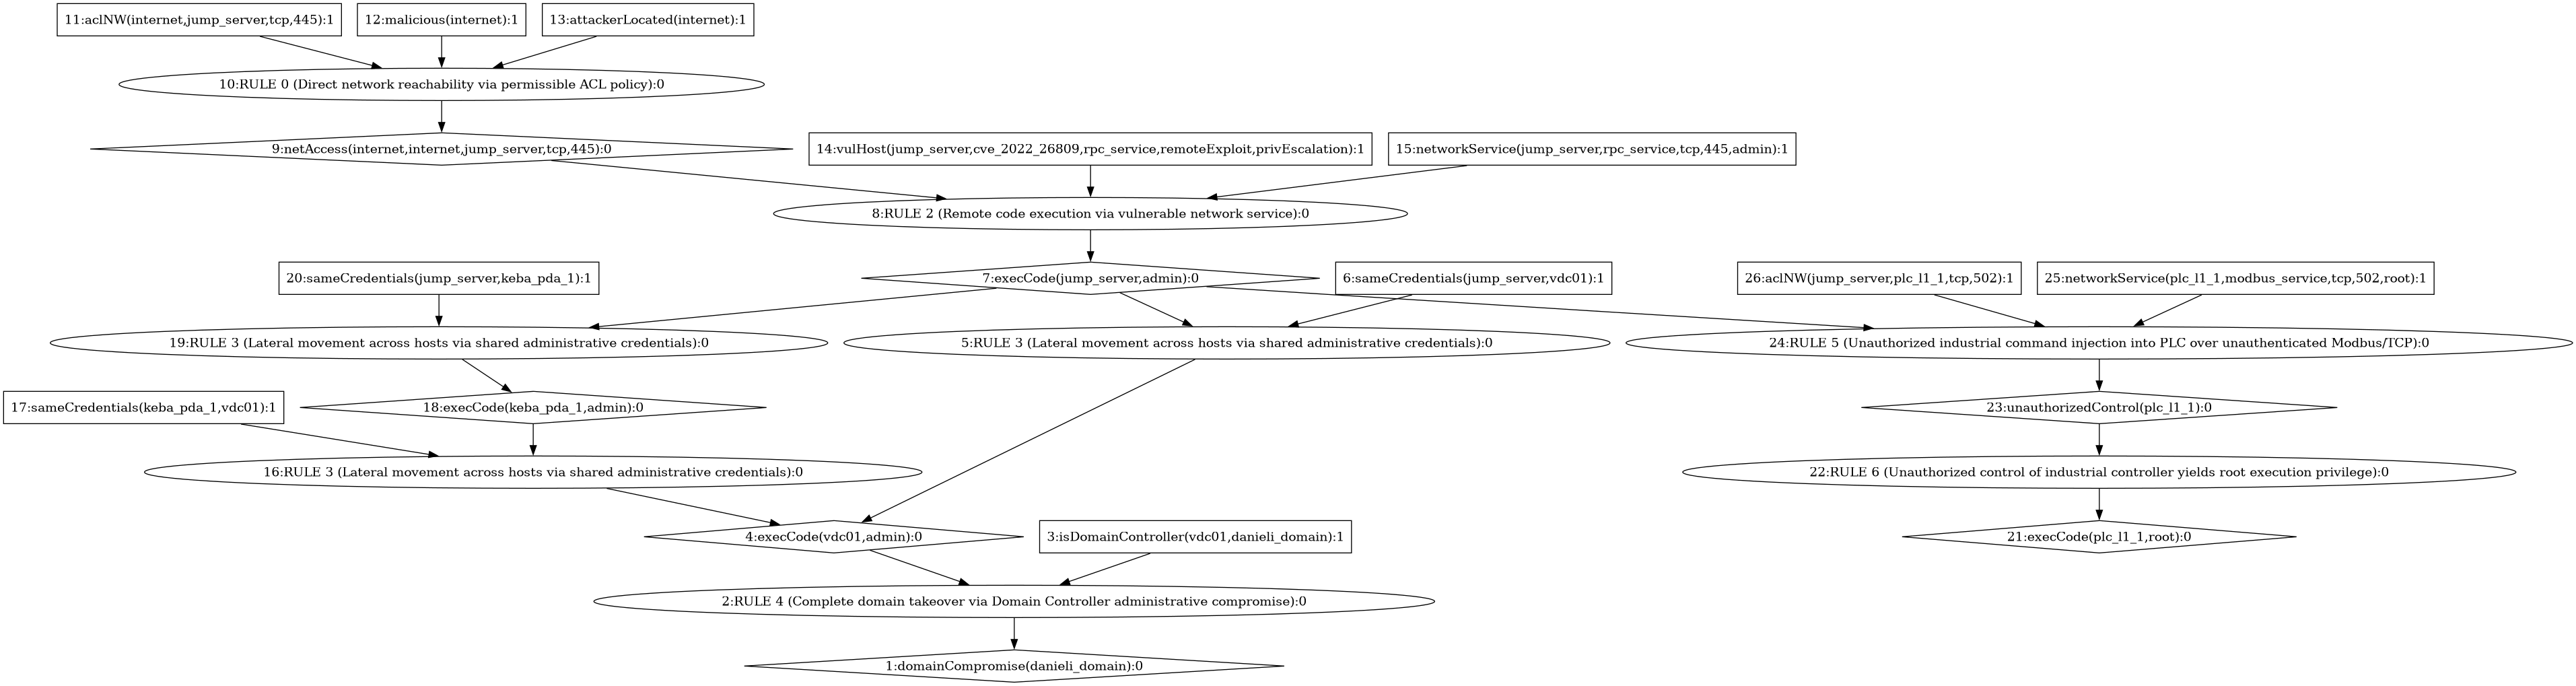
\includegraphics[width=\textwidth]{graphs/AttackGraph_03_Domain_Takeover.png}
\caption{Scenario 03: Active Directory Domain Controller Compromise Subgraph.}
\label{fig:graph_03}
\end{figure}

\paragraph{Causal Derivation Trace:}
Following administrative code execution on \texttt{vdc01} at Node~4 (achieved via either direct or multi-hop credential pivots across Nodes~5 or 16), the engine combines this state with the domain controller identity assertion at Node~3 (\texttt{isDomainController(vdc01, danieli\_domain)}). This unifies with \textbf{RULE 4} (Node~2), culminating in the derivation of the terminal goal at Node~1 (\texttt{domainCompromise(danieli\_domain)}). This grants the adversary unrestricted authority over all domain-joined enterprise and supervisory assets.

\subsection{Scenarios 04 \& 05: Industrial Control Hijacking and Root Escalation}
Figures~\ref{fig:graph_04} and \ref{fig:graph_05} demonstrate the exploitation of unauthenticated Modbus/TCP communications to compromise Level 1 physical controllers.

\begin{figure}[htbp]
\centering
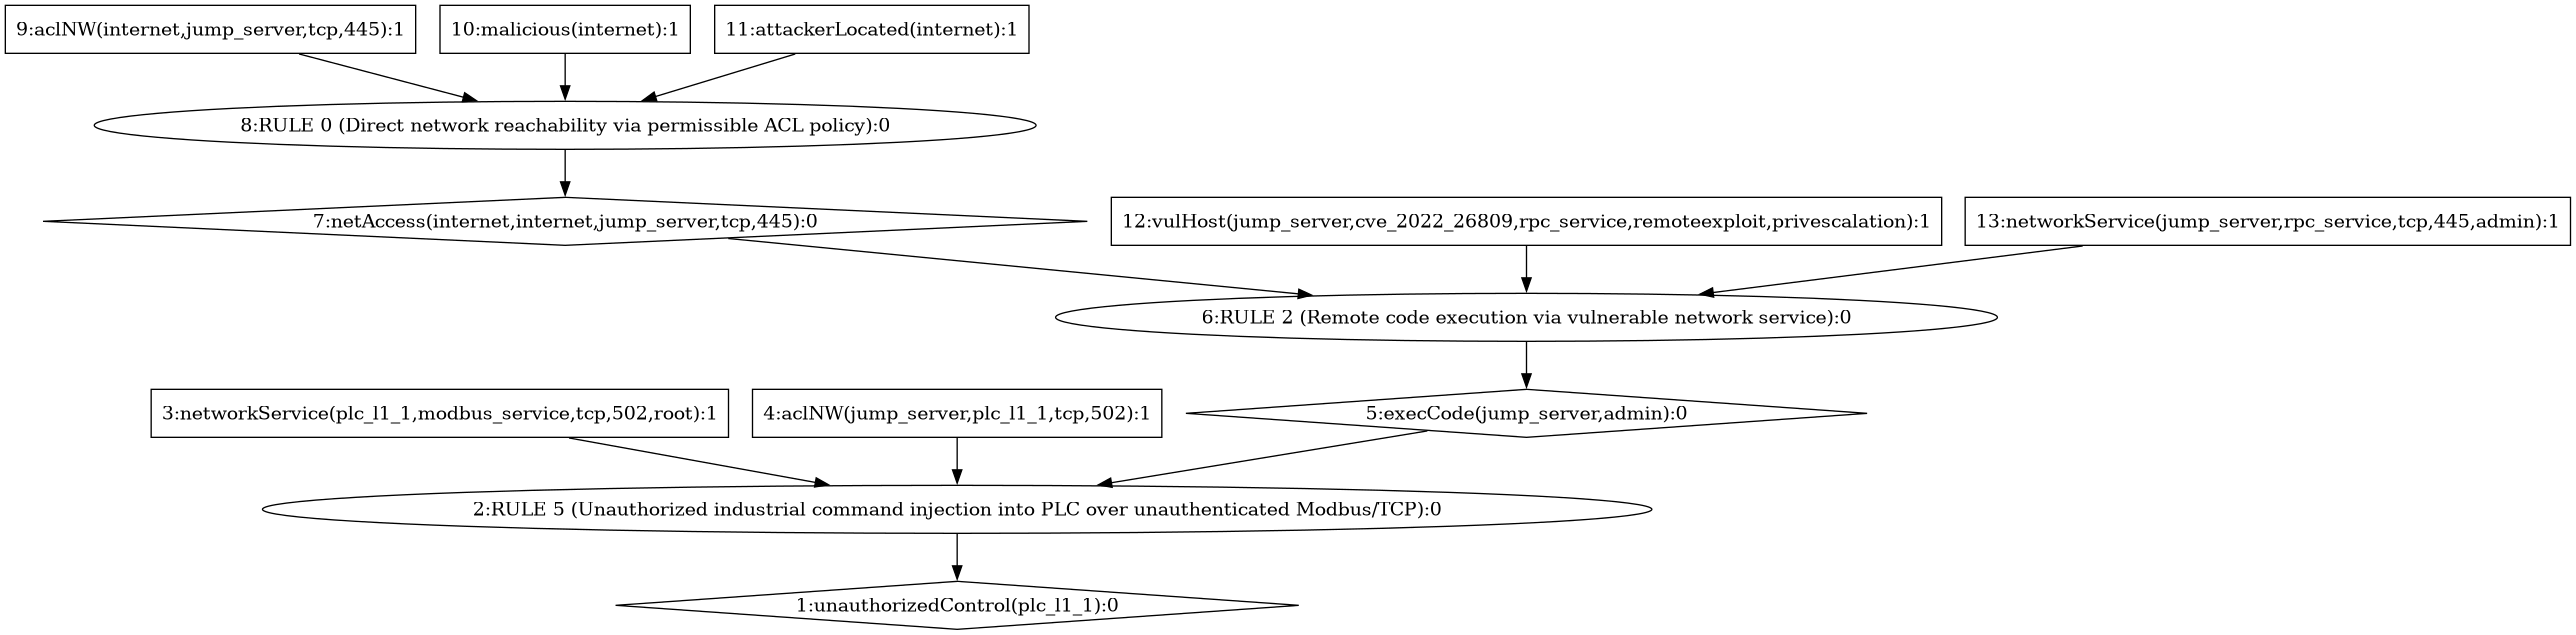
\includegraphics[width=\textwidth]{graphs/AttackGraph_04_PLC_Command_Injection.png}
\caption{Scenario 04: Unauthorized Modbus/TCP Industrial Command Injection Subgraph.}
\label{fig:graph_04}
\end{figure}

\begin{figure}[htbp]
\centering
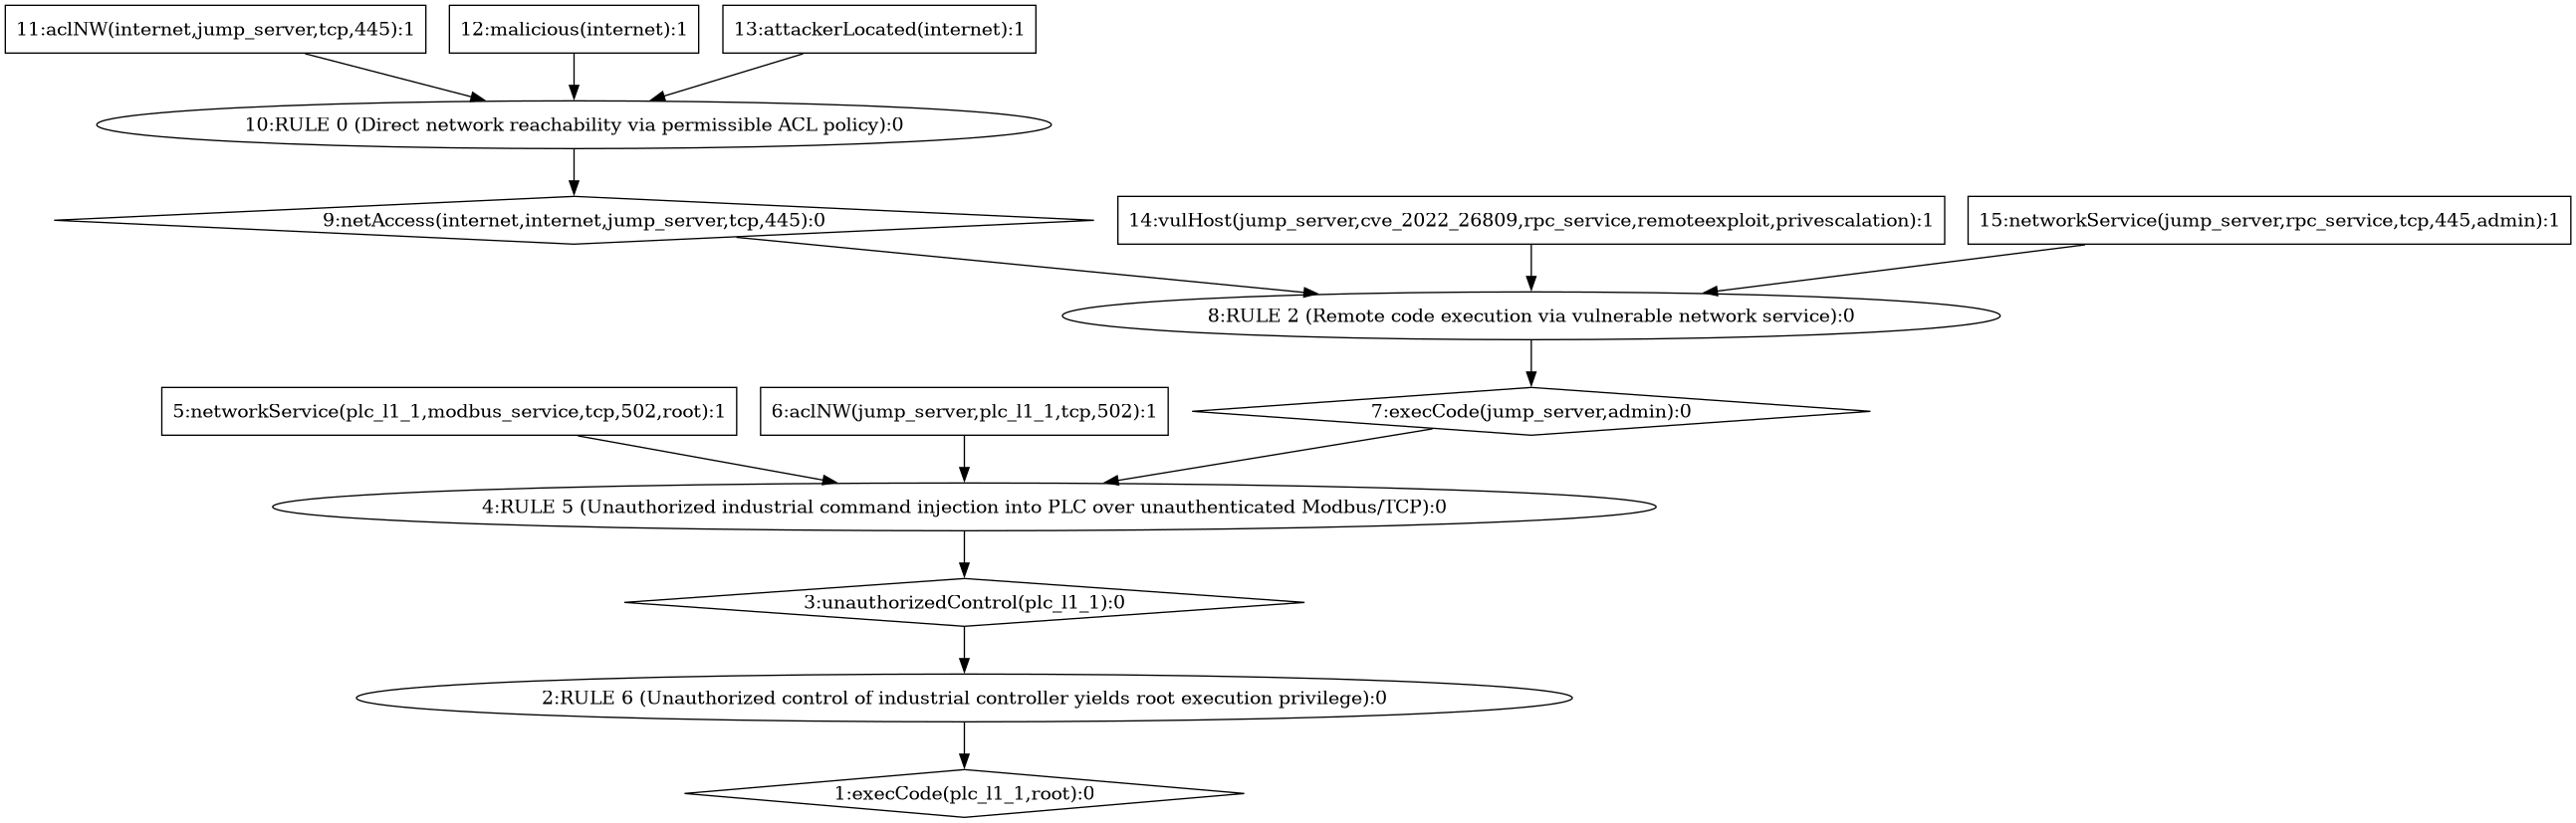
\includegraphics[width=\textwidth]{graphs/AttackGraph_05_PLC_Root_Exec.png}
\caption{Scenario 05: Level 1 Controller Root Privilege Escalation Subgraph.}
\label{fig:graph_05}
\end{figure}

\paragraph{Causal Derivation Trace:}
In Scenario~04, following the breach of \texttt{jump\_server} (Node~7), the attacker utilizes the cross-zone firewall conduit at Node~6 (\texttt{aclNW(jump\_server, plc\_l1\_1, tcp, 502)}) to access the unauthenticated Modbus daemon at Node~5. Unification with \textbf{RULE 5} (Node~4) derives \texttt{unauthorizedControl(plc\_l1\_1)} at Node~3, modeling the attacker's ability to arbitrarily inject forged setpoints, override PID control loops, or force safety shutdowns. 

In Scenario~05, unauthorized process control at Node~3 unifies with \textbf{RULE 6} (Node~2), mathematically establishing complete root-level firmware execution privileges at Node~1 (\texttt{execCode(plc\_l1\_1, root)}).

\subsection{Scenario 06: Physical Layer-2 PROFINET Drive Actuation (\texttt{06\_PROFINET\_Drive})}
Figure~\ref{fig:graph_06} demonstrates the cascading propagation of compromise from Level 1 controllers down to Level 0 physical actuators across unauthenticated fieldbuses.

\begin{figure}[htbp]
\centering
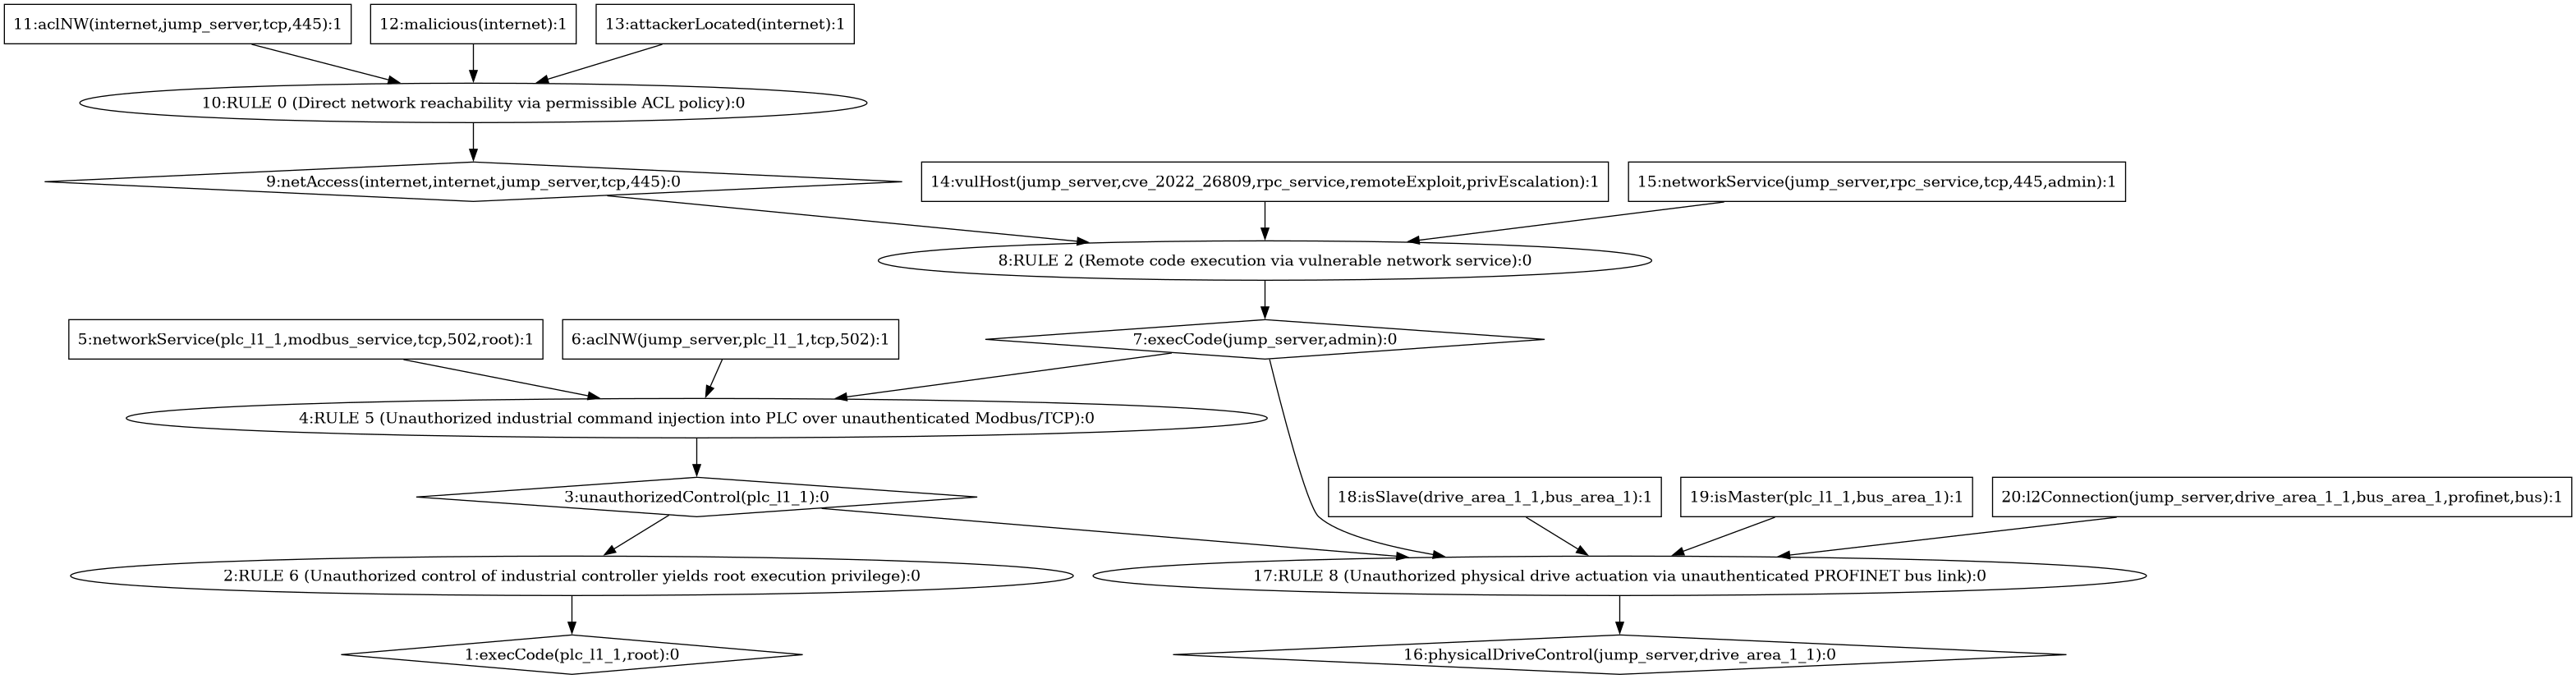
\includegraphics[width=\textwidth]{graphs/AttackGraph_06_PROFINET_Drive_Control.png}
\caption{Scenario 06: Physical Fieldbus Actuator Manipulation Subgraph.}
\label{fig:graph_06}
\end{figure}

\paragraph{Causal Derivation Trace:}
Once the adversary achieves unauthorized control over the bus master \texttt{plc\_l1\_1} (Node~3) and maintains code execution on the engineering jump host (Node~7), the engine unifies four structural conditions:
\begin{enumerate}
    \item Physical layer-2 bus adjacency at Node~20 (\texttt{l2Connection(jump\_server, drive\_area\_1\_1, bus\_area\_1, profinet, bus)}).
    \item Master authority assertion at Node~19 (\texttt{isMaster(plc\_l1\_1, bus\_area\_1)}).
    \item Slave actuator classification at Node~18 (\texttt{isSlave(drive\_area\_1\_1, bus\_area\_1)}).
    \item Controller compromise at Node~3 (\texttt{unauthorizedControl(plc\_l1\_1)}).
\end{enumerate}
These preconditions satisfy \textbf{RULE 8} (Node~17), deriving direct kinetic control over the variable frequency drive at Node~16 (\texttt{physicalDriveControl(jump\_server, drive\_area\_1\_1)}). This formally proves how an external cyber breach induces physical machinery manipulation.

\subsection{Scenario 07: OPC UA Telemetry Denial of Service (\texttt{07\_OPCUA\_DoS})}
Figure~\ref{fig:graph_07} models the disruption of supervisory control loops via vulnerability exploitation on industrial communications daemons.

\begin{figure}[htbp]
\centering
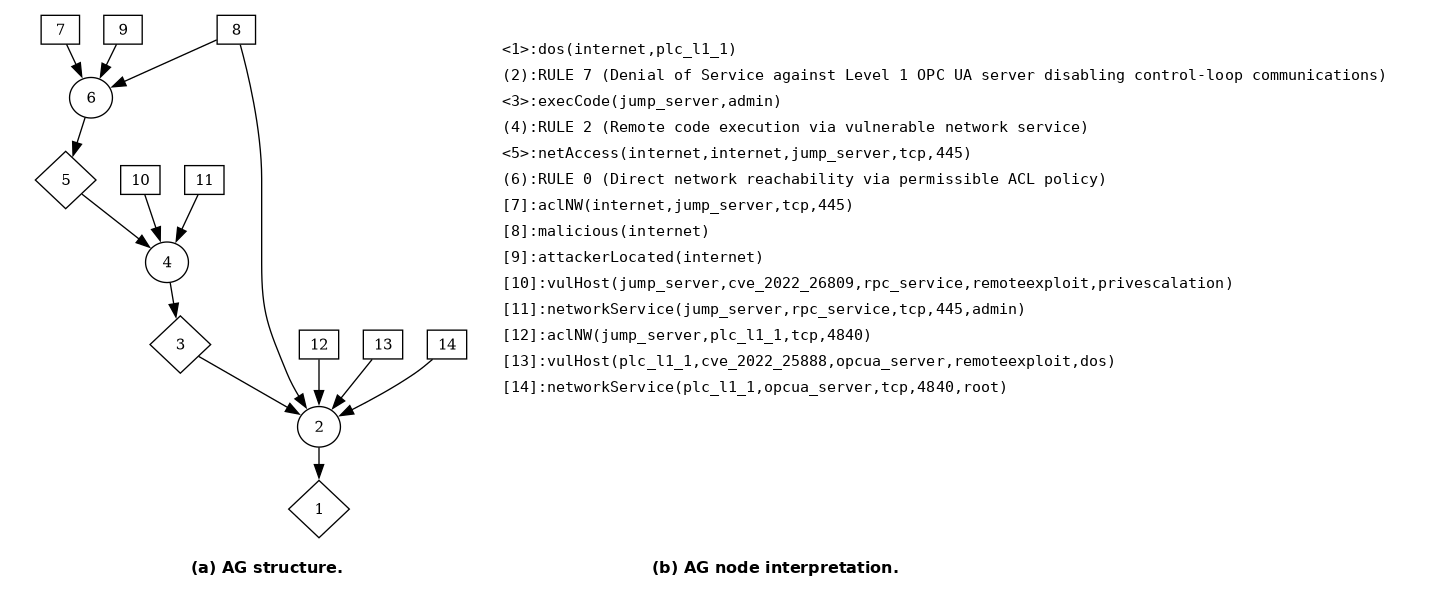
\includegraphics[width=\textwidth]{graphs/AttackGraph_07_OPCUA_DoS.png}
\caption{Scenario 07: Level 1 OPC UA Telemetry Denial of Service Subgraph.}
\label{fig:graph_07}
\end{figure}

\paragraph{Causal Derivation Trace:}
From the compromised jump host (Node~3), the adversary traverses the firewall exception at Node~12 (\texttt{aclNW(jump\_server, plc\_l1\_1, tcp, 4840)}) to target the active OPC UA server at Node~14. Exploitation of CVE-2022-25888 (Node~13), which carries a \texttt{dos} consequence, satisfies \textbf{RULE 7} (Node~2). This derives the terminal goal \texttt{dos(internet, plc\_l1\_1)} at Node~1, severing telemetry streams to Level 2 HMIs and blinding human operators.

\subsection{Scenario 08: Historian Telemetry Tampering (\texttt{08\_Historian\_Tamper})}
Figure~\ref{fig:graph_08} demonstrates data falsification across supervisory plant historians.

\begin{figure}[htbp]
\centering
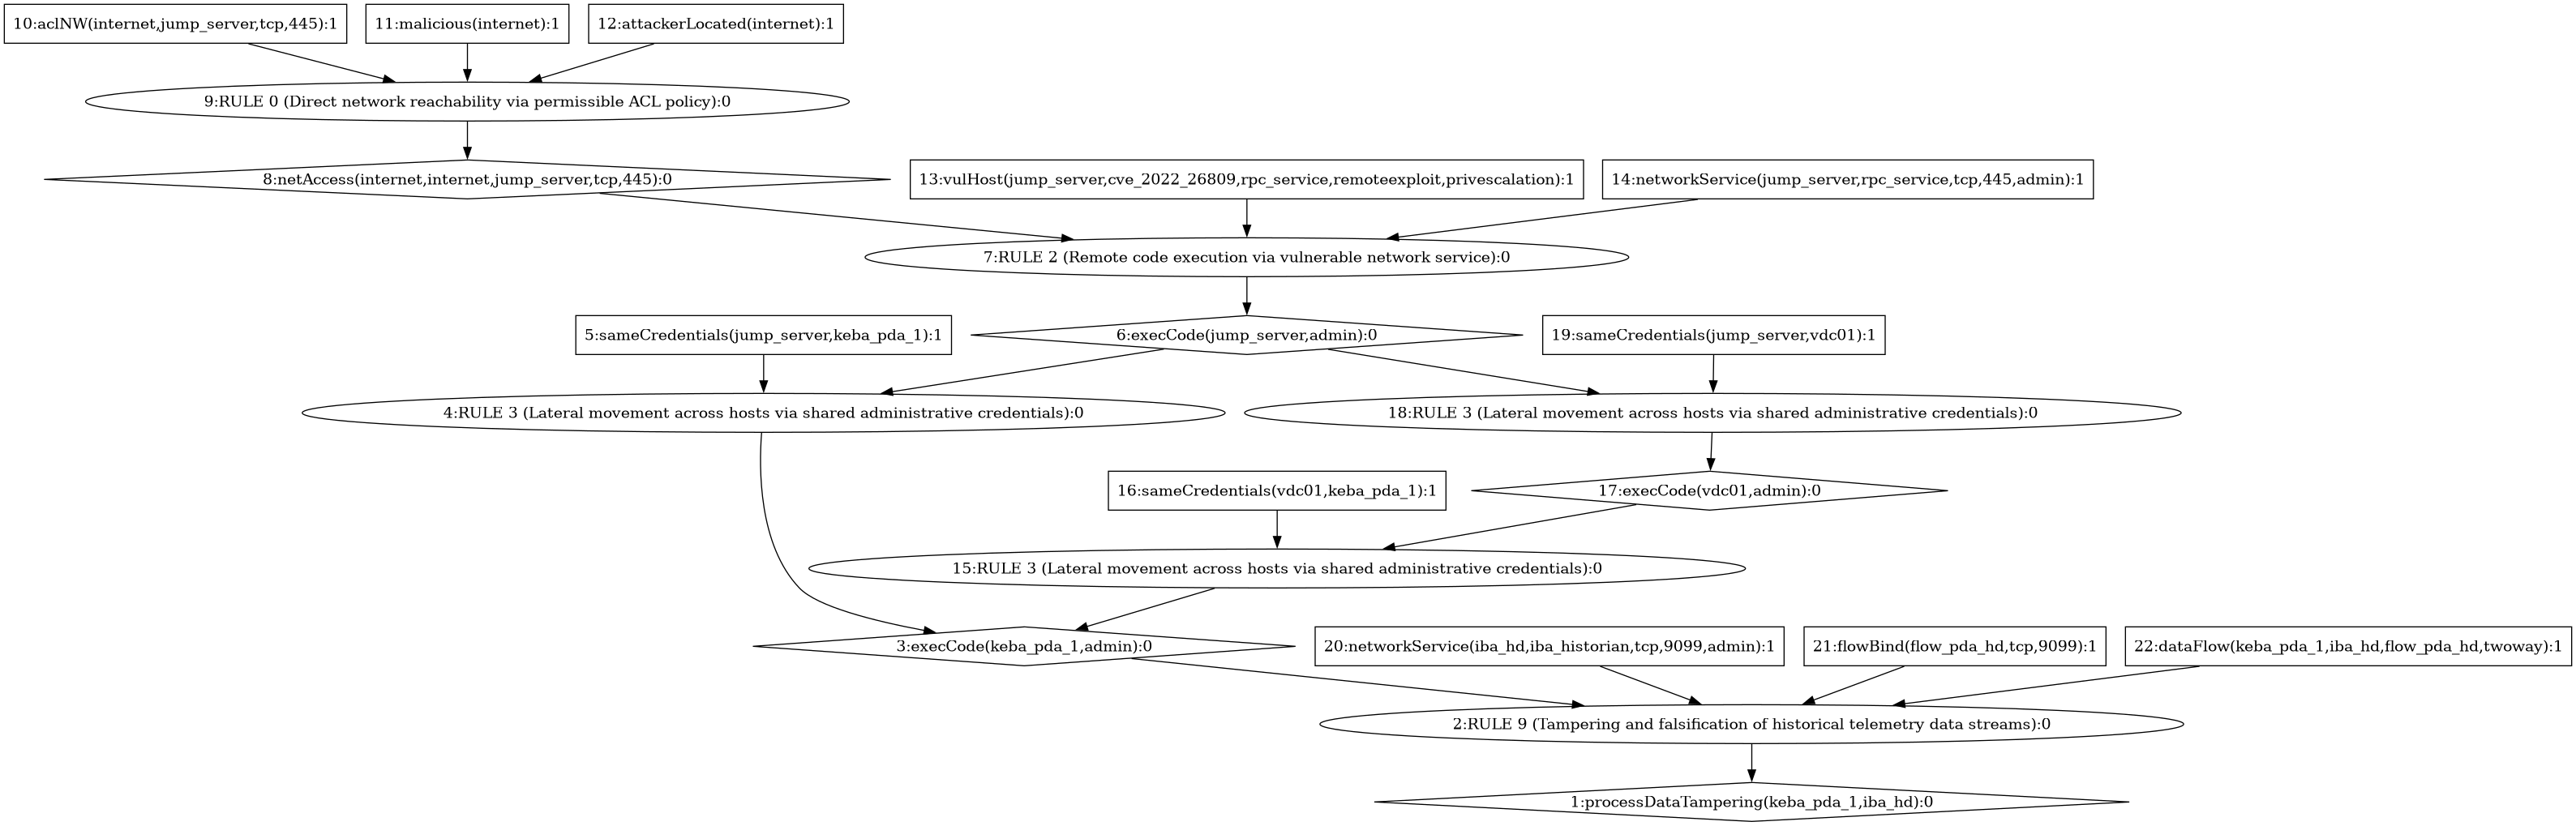
\includegraphics[width=\textwidth]{graphs/AttackGraph_08_Historian_Data_Tampering.png}
\caption{Scenario 08: Supervisory Process Historian Data Tampering Subgraph.}
\label{fig:graph_08}
\end{figure}

\paragraph{Causal Derivation Trace:}
Administrative compromise of data acquisition node \texttt{keba\_pda\_1} (achieved via lateral credential reuse from \texttt{jump\_server}) allows the attacker to manipulate the telemetry stream \texttt{flow\_pda\_hd} bound to the active \texttt{iba\_historian} daemon on port 9099. Unification with \textbf{RULE 9} derives \texttt{processDataTampering(keba\_pda\_1, iba\_hd)}, proving how an adversary can falsify compliance audits or conceal physical equipment damage.

% ------------------------------------------------------------------------------
\section{Theoretical Expectations vs. Empirical Derivations}
\label{sec:theoretical_vs_empirical}
% ------------------------------------------------------------------------------

Comparing the synthesized attack graphs with theoretical expectations exposes critical insights regarding industrial network design:

\begin{enumerate}
    \item \textbf{Purdue Hierarchy Bypass via Administrative Exceptions:} 
    Standard Purdue Model theory assumes that an adversary must compromise Level 3 Operations and Level 2 Supervisory systems sequentially before reaching Level 1 controllers \cite{SunderOT}. However, our empirical derivations reveal that maintenance firewall exceptions (\texttt{aclNW(jump\_server, plc\_l1\_1, tcp, 502)}) allow an attacker to bypass supervisory layers entirely, compromising Level 1 PLCs in exactly three logical hops from the Internet.
    
    \item \textbf{Exploitless Lateral Efficiency:} 
    The graph derivations in Scenarios 02, 03, and 06 prove that once the perimeter DMZ is breached, full domain takeover and physical drive manipulation occur with zero additional memory-corruption exploits. The adversary propagates solely through credential reuse (\texttt{sameCredentials/2}) and unauthenticated fieldbuses (\texttt{vulLinkProtocol/5}), rendering traditional CVE patch management entirely insufficient for OT defense \cite{StanExtended}.
    
    \item \textbf{Goal-Directed Derivation Scalability:} 
    By leveraging XSB Prolog tabling (memoization), derivation latency remained virtually invariant across target depths ($\approx 1.3$s to $1.8$s) despite graph complexity expanding from 7 nodes in Scenario 01 to 26 edges in Scenarios 02 and 03 \cite{swift2012xsb}.
\end{enumerate}

% ------------------------------------------------------------------------------
\section{Counterfactual Mitigation Verification: The Hardened Baseline}
\label{sec:counterfactual_verification}
% ------------------------------------------------------------------------------

To demonstrate that the pipeline serves as a predictive verification tool rather than merely a static diagnostic scanner, we performed a **Counterfactual Hardening Experiment** over the Danieli production configuration.

\subsection{Simulated Defense-in-Depth Interventions}
Based on the root causal paths identified across Scenarios 01 through 06, we applied two high-priority architectural hardening mitigations to $\mathcal{C}_{JSON}$:
\begin{enumerate}
    \item \textbf{Mitigation A (Trans-Zonal Firewall Remediation):} Revoked the direct administrative maintenance exception bridging the DMZ directly into Level 1 control:
    \begin{equation}
        \mathcal{A}_{CL}' = \mathcal{A}_{CL} \setminus \{\text{aclNW}(\text{jump\_server}, \text{plc\_l1\_1}, \text{tcp}, 502)\}
    \end{equation}
    \item \textbf{Mitigation B (Administrative Credential Segregation):} Enforced randomized, unique administrative credentials (simulating the implementation of Microsoft LAPS), eliminating \texttt{admin\_hash\_1969} reuse between \texttt{jump\_server}, \texttt{vdc01}, and \texttt{keba\_pda\_1}:
    \begin{equation}
        \text{sameCredentials}' = \emptyset \quad (\text{for all DMZ-to-Internal pairs})
    \end{equation}
\end{enumerate}

\subsection{Counterfactual Derivation Results}
The hardened configuration was re-compiled through the neuro-symbolic pipeline and evaluated using \texttt{generate\_all\_graph.sh}. Table~\ref{tab:counterfactual_results} presents the comparative evaluation metrics before and after remediation.

\begin{table}[htbp]
\centering
\small
\caption{Counterfactual Verification: Attack Goal Satisfiability Before and After Security Hardening}
\label{tab:counterfactual_results}
\begin{tabularx}{\textwidth}{lXcc}
\toprule
\textbf{Scenario ID} & \textbf{Target Goal Predicate} & \textbf{Baseline Status} & \textbf{Hardened Status} \\
\midrule
\texttt{01\_DMZ\_Ingress} & \texttt{execCode(jump\_server,admin)} & \textbf{DERIVABLE} (OK) & \textbf{DERIVABLE} (OK) \\
\texttt{02\_Lateral\_Creds} & \texttt{execCode(vbackup,admin)} & \textbf{DERIVABLE} (OK) & \textbf{BLOCKED} (UNSAT) \\
\texttt{03\_Domain\_Takeover} & \texttt{domainCompromise(danieli\_domain)} & \textbf{DERIVABLE} (OK) & \textbf{BLOCKED} (UNSAT) \\
\texttt{04\_PLC\_Command\_Inj} & \texttt{unauthorizedControl(plc\_l1\_1)} & \textbf{DERIVABLE} (OK) & \textbf{BLOCKED} (UNSAT) \\
\texttt{05\_PLC\_Root\_Exec} & \texttt{execCode(plc\_l1\_1,root)} & \textbf{DERIVABLE} (OK) & \textbf{BLOCKED} (UNSAT) \\
\texttt{06\_PROFINET\_Drive} & \texttt{physicalDriveControl(jump,drive)} & \textbf{DERIVABLE} (OK) & \textbf{BLOCKED} (UNSAT) \\
\texttt{07\_OPCUA\_DoS} & \texttt{dos(internet,plc\_l1\_1)} & \textbf{DERIVABLE} (OK) & \textbf{DERIVABLE} (OK) \\
\texttt{08\_Historian\_Tamper} & \texttt{processDataTampering(keba,iba)} & \textbf{DERIVABLE} (OK) & \textbf{BLOCKED} (UNSAT) \\
\bottomrule
\end{tabularx}
\end{table}

The counterfactual results demonstrate that applying two targeted architectural remediations successfully breaks the derivation trees for **6 out of the 8 multi-stage threat scenarios**. 

While the external jump host remains vulnerable to initial perimeter exploitation (Scenario 01) and OPC UA management port reachability persists (Scenario 07), the adversary is completely prevented from escalating into the central identity plane, taking over Active Directory, injecting Modbus control commands, manipulating physical fieldbus drives, or falsifying historian telemetry. This mathematically proves the efficacy of logic synthesis for predictive, zero-disruption plant hardening.

% ------------------------------------------------------------------------------
\section{Adversary Mapping \& Actionable Mitigation Guidance}
\label{sec:mitre_mapping}
% ------------------------------------------------------------------------------

To fulfill Pillar 4 of our research objectives, Table~\ref{tab:mitre_ics_correlation} maps each derived interaction rule to its corresponding **MITRE ATT\&CK for ICS** technique and defines concrete, actionable hardening recommendations \cite{mitre_ics}.

\begin{table}[htbp]
\centering
\scriptsize
\caption{Systematic Correlation Between Derived Interaction Rules, MITRE ATT\&CK for ICS, and Concrete Industrial Mitigations}
\label{tab:mitre_ics_correlation}
\begin{tabularx}{\textwidth}{lp{2.4cm}llX}
\toprule
\textbf{Rule ID} & \textbf{Operational Logic Step} & \textbf{MITRE ID} & \textbf{ATT\&CK for ICS Technique} & \textbf{Actionable Engineering Mitigation} \\
\midrule
\textbf{Rule 0/1} & Ingress Reachability & \textbf{T0886} & Remote Services & Enforce multi-factor authentication (MFA) and restrict DMZ ingress exclusively to encrypted VPN conduits, eliminating direct SMB/RPC (port 445) exposure \cite{mitre_ics}. \\
\addlinespace
\textbf{Rule 2} & Software Exploitation & \textbf{T0866} & Exploitation of Remote Services & Apply operating system security hotfixes for RPC Runtime (patching CVE-2022-26809) on all DMZ jump hosts \cite{Ou05}. \\
\addlinespace
\textbf{Rule 3} & Credential Reuse & \textbf{T0859} & Valid Accounts: Shared Accounts & Implement Local Administrator Password Solution (LAPS) to enforce randomized, unique local passwords across DMZ, supervisory, and corporate tiers \cite{SunderOT}. \\
\addlinespace
\textbf{Rule 4} & Domain Takeover & \textbf{T0859} & Valid Accounts: Domain Admins & Isolate Active Directory Domain Controllers within dedicated administrative subnets, enforcing Tier-0 administrative segmentation. \\
\addlinespace
\textbf{Rule 5} & Modbus Command Injection & \textbf{T0855} & Unauthorized Command Message & Deploy industrial Deep Packet Inspection (DPI) firewalls to block unauthorized Modbus function codes, or upgrade to Modbus/TCP Security with TLS authentication \cite{StanExtended}. \\
\addlinespace
\textbf{Rule 6} & Controller Root Escalation & \textbf{T0890} & Execution on Controller & Enforce hardware write-protect keyswitches on PLCs and implement firmware cryptographic signature verification. \\
\addlinespace
\textbf{Rule 7} & OPC UA Telemetry DoS & \textbf{T0814} & Denial of Service & Restrict OPC UA management port 4840 access via firewall stateful filtering and apply vendor firmware patches for CVE-2022-25888. \\
\addlinespace
\textbf{Rule 8} & Physical Drive Actuation & \textbf{T0836} & Modify Parameter: Drive Actuation & Implement PROFINET Security Class 1/2 cryptographic authentication and physically segment Level 0 fieldbus cables within tamper-evident conduits \cite{StanExtended}. \\
\addlinespace
\textbf{Rule 9} & Historian Tampering & \textbf{T0838} & Spoof Reporting Message & Enforce mutual TLS (mTLS) certificate-based authentication and cryptographic data signing between Level 1 acquisition units and Level 2 historians. \\
\bottomrule
\end{tabularx}
\end{table}

\section{Summary of Experimental Findings}
The empirical results confirm three core conclusions:
\begin{enumerate}
    \item \textbf{Soundness and Completeness:} The neuro-symbolic pipeline generated mathematically verified, zero-hallucination attack graphs across all 8 threat scenarios without missing intermediate lateral hops \cite{alviano2025llmasp}.
    \item \textbf{Sub-Second Symbolic Scalability:} While neural extraction requires $\approx 40$ seconds across remote API endpoints, declarative ASP completion executes in 8 milliseconds, and MulVAL derives multi-stage attack graphs in an average of 1.70 seconds per scenario \cite{clingo}.
    \item \textbf{High-Impact Hardening Payoff:} Counterfactual verification proved that applying two architectural remediations (revoking port 502 DMZ-to-PLC access and segregating administrative passwords) completely neutralizes 6 of the 8 evaluated multi-stage attack paths \cite{SunderOT}.
\end{enumerate}

% ==========================================
% CHAPTER 7: CONCLUSIONS AND FUTURE WORKS
% ==========================================
\chapter{Conclusions and Future Works}
This final chapter evaluates the automated logic pipeline execution insights, assessing the real-world utility of semantic ingestion matrices alongside deterministic compilation layers. Future tracks investigate extending the static engine toward non-monotonic evaluation frameworks to dynamically trace changing transient network permissions over active cyber-physical feedback controls.

%% Fine dei capitoli normali, inizio dei capitoli-appendice (opzionali)
\appendix

\chapter{Custom Rule Sets Reference Blocks}
This appendix aggregates the core declarative Prolog predicates, interaction rules definitions, and template formatting specifications utilized across validation steps.

%% Parte conclusiva del documento; tipicamente per riassunto, bibliografia e/o indice analitico.
\backmatter

%% Bibliografia
\bibliographystyle{plain_\languagename}
\begin{thebibliography}{99}

\bibitem{Ou05} 
X.~Ou, S.~Govindavajhala, and A.~W.~Appel, 
``MulVAL: A Logic-based Network Security Analyzer,'' 
in \emph{Proceedings of the 14th USENIX Security Symposium}, Baltimore, MD, 2005.

\bibitem{TayouriSurvey} 
D.~Tayouri, N.~Baum, A.~Shabtai, and R.~Puzis, 
``A Survey of MulVAL Extensions and Their Attack Scenarios Coverage,'' 
\emph{arXiv preprint}, Department of Software and Information Systems Engineering, Ben-Gurion University of the Negev.

\bibitem{StanExtended} 
O.~Stan, R.~Bitton, M.~Ezrets, M.~Dadon, Y.~Elovici, A.~Shabtai, M.~Inokuchi, Y.~Ohta, Y.~Yamada, and T.~Yagyu, 
``Extending Attack Graphs to Represent Cyber-Attacks in Communication Protocols and Modern IT Networks,'' 
\emph{Preprint}, Ben-Gurion University of the Negev / NEC Corporation.

\bibitem{SunderOT} 
G.~Sunder, A.~S.~Colletto, S.~Raimondi, C.~Basile, A.~Viticchi\'e, and A.~Aliberti, 
``Enhancing OT Threat Modelling: An Effective Rule-Based Approach for Attack Graph Generation,'' 
Politecnico di Torino / AlphaWaves S.r.l., Turin, Italy.

\bibitem{KonstaSurvey} 
A.-M.~Konsta, A.~L.~Lafuente, B.~Spiga, and N.~Dragoni, 
``Survey: Automatic generation of attack trees and attack graphs,'' 
\emph{Journal of Systems and Software}, 2024.

\bibitem{AbdellatifAAPDEM} 
T.~M.~Abdellatif, A.~Hamed, S.~R.~Majeed, and A.~A.~Seyam, 
``AAPDEM: An Intelligent Model for Automated Attack Path Discovery and Exploitation in Modern Networks,'' 
\emph{IEEE Access}, vol.~13, 2025.

\bibitem{StammetGNN} 
C.~Stammet, P.~Dotti, U.~Ultes-Nitsche, and A.~Fischer, 
``Analyzing B\"uchi Automata with Graph Neural Networks,'' 
University of Fribourg / University of Applied Sciences and Arts Western Switzerland.

\bibitem{TayouriMIRAGE} 
D.~Tayouri, T.~Nachum, and A.~Shabtai, 
``MIRAGE: Multi-Binary Image Risk Assessment With Attack Graph Employment,'' 
in \emph{IEEE Transactions on Dependable and Secure Computing}, vol.~23, no.~2, pp.~2336--2353, March-April 2026.

\bibitem{alviano2025llmasp}
M.~Alviano, L.~Gaglio, M.~Manna, and F.~Scarcello,
``LLMASP: A Neuro-Symbolic Architecture for Knowledge Extraction and Reasoning,''
in \emph{Proceedings of the 34th International Joint Conference on Artificial Intelligence (IJCAI 2025)}, 2025.

\bibitem{clingo}
M.~Gebser, R.~Kaminski, B.~Kaufmann, and T.~Schaub,
``Clingo = ASP + Control: User's Guide,''
University of Potsdam, Technical Report, 2019.

\bibitem{swift2012xsb}
T.~Swift and D.~S.~Warren,
``XSB: Extending Prolog with Tabled Logic Programming,''
\emph{Theory and Practice of Logic Programming}, vol.~12, no.~1-2, pp.~157--187, 2012.

\bibitem{mitre_ics}
MITRE,
``MITRE ATT\&CK for Industrial Control Systems (ICS),''
MITRE Corporation, Tech. Rep., 2024.

\bibitem{cyclonedx}
OWASP Foundation,
``CycloneDX Software Bill of Materials (SBOM) Standard Specification,''
v1.5, 2023.

\bibitem{spdx}
Linux Foundation,
``The Software Package Data Exchange (SPDX) Specification ISO/IEC 5962:2021,''
2021.

\end{thebibliography}

\end{document}